\chapter{Βασικές λειτουργίες}
\label{ch:foundation}

Το κεφάλαιο αναφέρεται σε ορισμένες βασικές μονάδες της υλοποίησης

%Όπως συζητείται στο κεφάλαιο \nref{}
Ο μικροελεγκτής διαθέτει εσωτερική μνήμη EEPROM η οποία μπορεί να χρησιμοποιηθεί
για την αποθήκευση δεδομένων που διατηρούνται μεταξύ διαδοχικών απενεργοποιήσεων
του και η οποία, στην περίπτωση του ATmega328P, είναι χωρητικότητας 1KiB.
Η υλοποίηση έχει την ανάγκη για τη .. των αρχείων διεπαφής.
Οι απαιτήσεις των αρχείων αυτών σε αποθηκευτικό χώρο είναι δύσκολο να
ικανοποιηθούν είτε από τη μνήμη EEPROM είτε τη Flash του μικροελεγκτή, καθώς η
πρώτη ανέρχεται μόλις στο 1KiB, ενώ η δεύτερη, στα 32KiB, η οποία
χρησιμοποιείται, κατά κύριο λόγο, για την αποθήκευση του λογισμικού
(προγράμματος) του μικροελεγκτή και θα ήταν δύσκολο να χρησιμοποιηθεί και για
τα αρχεία της διεπαφής.
Για το λόγο αυτό επιλέγεται ένα ολοκληρωμένο μνήμης Flash χωρητικότητας 1024bit
(128KiB) για την αποθήκευση των αρχείων της διεπαφής (ιστοσελίδα, αρχείο
css \etc{.}). Τα δεδομένα της συγκεκριμένης μνήμης αρχικοποιούνται (δηλαδή,
εγγράφονται) σε ένα στάδιο πριν τον τελικό προγραμματισμό της συσκευής και, κατά
τη διάρκεια της κανονικής της λειτουργίας, η μνήμη χρησιμοποιείται μόνο για
ανάγνωση (βλ. \nameref{subsec:external-memory} σ.~%
\pageref{subsec:external-memory}).

Επιπλέον, ορίζεται μία εφεδρική μνήμη η οποία χρησιμεύει για την αποθήκευση των
ρυθμίσεων της συσκευής, δηλαδή τιμών που τίθενται από το χρήστη και επηρεάζουν
τη συμπεριφορά της συσκευής (βλ. σ.~\pageref{subsec:backup-memory}). Ο λόγος
ύπαρξής της είναι η διατήρηση των ρυθμίσεων μεταξύ διαδοχικών επανεκκινήσεων της
συσκευής. Χαρακτηρίζεται ως «εφεδρική» επειδή τα δεδομένα που εναποτίθενται σε
αυτήν θεωρούνται έγκυρα όσο η εφεδρική τροφοδοσία της συσκευής είναι διαθέσιμη,
ενώ επαναφέρονται στις προκαθορισμένες τιμές (τις εργοστασιακές ρυθμίσεις)
εφόσον και αυτή (επιπροσθέτως της κύριας τροφοδοσίας) απενεργοποιηθεί προσωρινά.
Η εφεδρική τροφοδοσία πρόκειται για μία συστοιχία συσσωρευτών (μπαταρία) που
επιτρέπει στο ρολόι πραγματικού χρόνου (RTC) να λειτουργεί κατά τα διαστήματα
που η συσκευή είναι αποσυνδεδεμένη από την κύρια τροφοδοσία (δηλαδή, όταν η
συσκευή είναι απενεργοποιημένη).

Στη συνέχεια αναλύεται το λογισμικό που είναι υπεύθυνο για τη διαχείριση των
μετρήσεων, το Ημερολόγιο (\pageref{sec:log}). Το Ημερολόγιο αναλαμβάνει την
αποθήκευση και ανάκτηση εγγραφών οι οποίες περιέχουν, υποχρεωτικά, ημερομηνία%
\slash{}ώρα και ένα πλήθος επιπρόσθετων Byte. Οι εγγραφές επιστρέφονται σε
φθίνουσα σειρά βάσει της ημερομηνίας\slash{}ώρας κάθε εγγραφής ενώ η ανάκτησή
τους υλοποιείται με τρόπο που διευκολύνει τη σελιδοποίηση των εγγραφών στο
πλαίσιο αναζητήσεων (βλ. \nameref{subsec:network:measurement} σ.~%
\pageref{subsec:network:measurement}).

Ο αποθηκευτικός χώρος των εγγραφών του Ημερολογίου έχει επιλεγεί να είναι η
εσωτερική μνήμη EEPROM του μικροελεγκτή (1 KiB). Πρακτικά, αυτό σημαίνει ότι το
Ημερολόγιο είναι ρυθμισμένο να διατηρεί τις 90 πλέον πρόσφατες μετρήσεις,
αφήνοντας μερικά Byte (34) για ενδεχόμενα άλλα δεδομένα.

Κατόπιν, ακολουθεί περιγραφή της διευθέτησης και χειρισμού του ρολογιού
πραγματικού χρόνου (\te{RTC -- Real-Time Clock}), ένα ολοκληρωμένο που παρέχει
στη συσκευή τη δυνατότητα αναγνώρισης της τρέχουσας ημερομηνίας\slash{}ώρας
(βλ. \nameref{sec:rtc} σ.~\pageref{sec:rtc}). Στο παρόν στάδιο της υλοποίησης,
το ολοκληρωμένο χρησιμοποιείται για την αναγνώριση του χρόνου που έχει παρέλθει
από την τελευταία μέτρηση του Ημερολογίου ώστε να αποφασίζεται εάν πρέπει να
εκκινηθεί νέος κύκλος μετρήσεων. Ο σχετικός έλεγχος πραγματοποιείται κάθε 8s από
ξεχωριστή μονάδα, όταν ο μικροελεγκτής αφυπνίζεται από εσωτερικό κύκλωμά
του, το \te{Watch-Dog Timer} (WDT).

Η υπεύθυνη μονάδα για την εκτέλεση των μετρήσεων -- όπου στο πλαίσιο της
υλοποίησης περιλαμβάνουν μόνο τη θερμοκρασία -- είτε με αυτόματο τρόπο είτε μη
περιγράφεται στην \nameref{sec:task} (σ.~\pageref{sec:task}). Στο πλαίσιο της,
παρέχεται, επιπροσθέτως, η δυνατότητα εκτίμησης του χρόνου ολοκλήρωσης της
τρέχουσας εργασίας (είτε αυτή αναφέρεται σε μεμονωμένη ή αλληλουχία μετρήσεων,
είτε σε απλή μετακίνηση της κεφαλής) το οποίο αξιοποιείται κατά την απόκριση σε
ορισμένα αιτήματα (βλ. \nameref{sec:network:impl-resources} σ.~%
\pageref{sec:network:impl-resources}).

Τέλος, αναλύονται οι δίαυλοι και το λογισμικό οδήγησης που χρησιμοποιούνται για
την επικοινωνία μεταξύ του μικροελεγκτή και των διαφόρων εξωτερικών
ολοκληρωμένων. Συνολικά, γίνεται χρήση των διαύλων 1-Wire, Ι\tsup{2}C και SPI
(βλ. \nameref{sec:buses} σ.~\pageref{sec:buses}).

%    Μνήμη προγράμματος
%    Εξοικονόμηση ενέργειας

\section{Μνήμες αποθήκευσης}

\subsection{Αρχεία διεπαφής}
\label{subsec:external-memory}

Κρίνεται σκόπιμη η ύπαρξη ενός αφιερωμένου αποθηκευτικού μέσου για την εναπόθεση
των αρχείων της διεπαφής της συσκευής (ιστοσελίδα, κώδικας javascript \etc{.} --
βλ. \nameref{subsec:network:files} σ.~\pageref{subsec:network:files}) καθώς οι,
εσωτερικά, διαθέσιμες μνήμες του μικροελεγκτή -- 32KiB μνήμη προγράμματος και
1KiB μνήμη EEPROM -- θεωρείται ότι αδυνατούν να τα υποστηρίξουν ή θα έθεταν
αισθητούς περιορισμούς στο μέγεθός τους και, συνεπώς, στη λειτουργικότητα της
διεπαφής.

Για το σκοπό αυτό, επιλέγεται το ολοκληρωμένο 25LC1024 το οποίο διαθέτει 128KiB
μνήμη EEPROM, χωρισμένη σε τέσσερις τομείς των 32KiB με 128 σελίδες ο καθένας,
με δυνατότητα εγγραφής σε επίπεδο Byte ή σελίδας και διασύνδεση μέσω διαύλου SPI
\parencite[1]{25lc1024}. Για λεπτομέρειες σχετικά με το δίαυλο SPI, βλ. σ.~%
\pageref{subsec:spi}. Κρίνεται ότι η χωρητικότητά του είναι υπεραρκετή για τις
τρέχουσες, ή άμεσα μελλοντικές, ανάγκες της υλοποίησης.
Στο παρόν στάδιο της υλοποίησης, η αποθήκευση των αρχείων στη μνήμη γίνεται σε
αυθαίρετα επιλεγμένες διευθύνσεις μνήμης, οι οποίες δηλώνονται κατά τη σύνταξη
του προγράμματος, ενώ τα αρχεία είναι αδύνατο να μεταβληθούν μέσα από την
υλοποίηση.

Η πρόσβαση της μνήμης του ολοκληρωμένου για την ανάγνωση και εγγραφή των κελιών
της γίνεται μέσω ορισμένων εντολών. Το σύνολο των εντολών μπορεί να χωριστεί σε
τρεις κατηγορίες· εντολές ανάγνωσης, εγγραφής και ειδικής χρήσης, καθεμία από
τις οποίες μελετάται ξεχωριστά. Στη γενική τους μορφή, όλες οι εντολές
περιγράφονται από τους ακόλουθους κανόνες:
\begin{lstlisting}
command     = instruction_code [ load ]
load        = memory_cell | octet
memory_cell = address *octet
\end{lstlisting}
Οι κωδικοί εντολών έχουν μήκος 8bit ενώ οι διευθύνσεις, 24bit εκ των οποίων τα
πρώτα 7 αγνοούνται από το ολοκληρωμένο καθώς τα υπολειπόμενα 17 είναι ικανά για
την αναφορά στις 128KiB διαθέσιμες θέσεις \parencite[6--7]{25lc1024}. Σαφώς,
τα πραγματικά μέρη που συνθέτουν την εκάστοτε εντολή εξαρτώνται από τον κωδικό
και, συνεπώς, τη λειτουργία της. Για παράδειγμα, η διεύθυνση κελιού μνήμης
(\te{\verb~address~}) έχει νόημα για τις εντολές ανάγνωσης, εγγραφής και
απαλοιφής μέρους της μνήμης, ενώ η απαλοιφή όλων των δεδομένων της μνήμης
(\te{Chip Erase}) απαιτεί μόνο τον κωδικό της (\te{\verb~instruction\_code~}).

Ωστόσο, όλες οι εντολές προϋποθέτουν ότι το 25LC1024 βρίσκεται σε κατάσταση
ετοιμότητας (δηλαδή, όχι σε κατάσταση χαμηλής κατανάλωσης ισχύος), ενώ ενδέχεται
να ισχύουν επιπρόσθετοι περιορισμοί, ανάλογα με την εντολή
\parencite[17]{25lc1024}.


\subsubsection{Ανάγνωση}
\label{ssubsec:25lc1024:read-commands}

Οι εντολές ανάγνωσης επιτρέπουν την ανάκτηση δεδομένων από τα κελιά της μνήμης
καθώς και την τιμή του καταχωρητή κατάστασης SR (\te{Status Register}) -- του
μοναδικού καταχωρητή του ολοκληρωμένου -- ο οποίος παρέχει στοιχεία για την
πορεία ενδεχόμενων εγγραφών και έλεγχο γύρω από την ενεργοποίηση της εγγραφής
(περισσότερα βλ. \nameref{ssubsec:25lc1024:write-protect}
σ.~\pageref{ssubsec:25lc1024:write-protect}).

Σύμφωνα με τη \textcite[6]{25lc1024}, το ολοκληρωμένο αγνοεί τις απόπειρες
ανάγνωσης μνήμης όταν βρίσκεται σε εξέλιξη εγγραφή δεδομένων, δηλαδή όσο η
ένδειξη WIP (\te{Write-In-Progress}) του καταχωρητή κατάστασης βρίσκεται σε
λογικό 1.

Ως εντολές ανάγνωσης μπορούν να χαρακτηριστούν οι ακόλουθες:
\begin{description}
    \item[READ [0x03{]}] Επιστρέφει το \te{Byte} της μνήμης που βρίσκεται στην
    προσδιοριζόμενη διεύθυνση και συνεχίζει με κάθε επόμενο για διαδοχικούς
    παλμούς της ίδιας εντολής, αυτομάτως μεταβαίνοντας στη διεύθυνση 0 ως το
    επόμενο \te{Byte} της τελευταίας διεύθυνσης \parencite[6--7]{25lc1024}.
    Προφανώς, η σύνταξη της εντολής απαιτεί διεύθυνση και τουλάχιστον ένα
    \te{Byte} δεδομένων.

    \item[RDSR [0x05{]}] (\te{ReaD Status Register}) Επιστρέφει την τιμή του
    καταχωρητή κατάστασης του ολοκληρωμένου και απαιτεί, επιπροσθέτως του
    κωδικού εντολής, ένα \te{Byte} \parencite[10]{25lc1024}.

    \item[RDID [0xAB{]}] (\te{ReaD ID}) Επιστρέφει το αναγνωριστικό της συσκευής
    και την αφυπνίζει από την κατάσταση χαμηλής κατανάλωσης ισχύος, εάν έχει
    τεθεί σε αυτήν. Η εντολή απαιτεί την αποστολή 24bit διεύθυνσης (τα οποία
    χρησιμοποιούνται για την προετοιμασία του ολοκληρωμένου, χωρίς να έχει
    ιδιαίτερη σημασία η τιμή τους), και ένα \te{Byte} για την επιστροφή του
    αναγνωριστικού (ή «υπογραφής») του \parencite[17]{25lc1024}
    \label{ssubsec:25lc1024:read-commands:rdid}.

    Για την εντολή μετάπτωσης σε κατάσταση χαμηλής κατανάλωσης ισχύος, βλ.
    \nameref{ssubsec:25lc1024:special-commands} (σ.~%
    \pageref{ssubsec:25lc1024:special-commands}).
\end{description}


\subsubsection{Εγγραφή και προστασία}
\label{ssubsec:25lc1024:write-protect}

Ως εγγραφή νοείται τόσο η αποστολή δεδομένων (Byte) από το μικροελεγκτή με
προορισμό τον καταχωρητή κατάστασης SR του ολοκληρωμένου ή συγκεκριμένες θέσεις
της μνήμης EEPROM, είτε η \emph{απαλοιφή} των δεδομένων από τα κελιά της μνήμης
και την επαναφορά τους στην προκαθορισμένη τιμή 0xFF (\te{erase})
\parencite[6--7]{25lc1024}.

Ωστόσο, για την αποφυγή μη εσκεμμένων (τυχαίων) εγγραφών στις θέσεις μνήμης με
αποτέλεσμα την αλλοίωση των δεδομένων, το ολοκληρωμένο απαιτεί τη δήλωση της
πρόθεσης για εγγραφή. Επιπλέον, παρέχονται δύο επιπρόσθετα επίπεδα προστασίας
ώστε να μειώνεται περαιτέρω η πιθανότητα ακούσιας τροποποίησης των δεδομένων από
αστοχίες υλικού και εξωτερικών παρεμβολών.

\paragraph{Μανδαλωτής WEL} Αρχικά, προκειμένου να εκτελεστεί οποιαδήποτε εντολή
εγγραφής, απαιτείται να προηγηθεί η αποστολή της εντολής WREN
(\te{WRite ENable}) ώστε να ενεργοποιηθεί ο μανδαλωτής WEL (\te{Write-Enable
Latch}) \parencite[6]{25lc1024}.
Κατόπιν, απενεργοποιείται η γραμμή \nbar{CS} (τίθεται σε λογικό 1) και
ενεργοποιείται ξανά (λογικό 0) για την αποστολή της εντολής εγγραφής. Ο
μανδαλωτής WEL απενεργοποιείται είτε αυτόματα με την ολοκλήρωση της εγγραφής
ή κατά την αρχική τροφοδοσία του ολοκληρωμένου με τάση (\te{power-on}) είτε
μέσω της, ειδικής για αυτόν τον σκοπό, εντολής WRDI (\te{WRite DIsable})
\parencite[9]{25lc1024}. Αυτό το επίπεδο προστασίας είναι το μοναδικό που
εφαρμόζεται υποχρεωτικά.

\begin{table}
    \caption{
    \label{tab:25lc1024:bp-bits}}
    \begin{center}\begin{tabu} spread 0pt {*2{X[-1,C]} X[2,L]}
    \rowfont\bfseries
    BP1 &   BP0 & Προστατευμένη περιοχή                                       \\
    \hline
      0 &     0 & Καμία                                                       \\
      0 &     1 & 3\tsup{ος} τομέας (0x18000--0x1FFFF)                        \\
      1 &     0 & 2\tsup{ος} και 3\tsup{ος} τομέας (0x10000--0x1FFFF)         \\
      1 &     1 & Όλοι οι τομείς (0x00000--0x1FFFF)                           \\
    \end{tabu}\end{center}

    Βασισμένο \fullcite[11]{25lc1024:bp-bits}
\end{table}

\paragraph{Προστατευμένες περιοχές} Ως ένα επιπρόσθετο επίπεδο ασφαλείας είναι
δυνατό να οριστεί, μέσω των \te{bit} BP1:0 του καταχωρητή SR, ποιος συνδυασμός
τομέων θα είναι «προστατευμένος από εγγραφή», με την έννοια ότι η εγγραφή στις
θέσεις μνήμης αυτών των τομέων απενεργοποιείται, εκτός και εάν προηγηθεί
τροποποίηση αυτής της ρύθμισης σε προγενέστερο χρόνο της εντολής εγγραφής
\parencite[10,12]{25lc1024}. Οι δυνατοί συνδυασμοί παρουσιάζονται στον πίνακα
\ref{tab:25lc1024:bp-bits}.

\paragraph{Προστασία καταχωρητή SR} Το τελευταίο στάδιο προστασίας αφορά τον
καταχωρητή SR και συμπεριλαμβάνει το χειρισμό του ακροδέκτη \nbar{WP} του
ολοκληρωμένου επιπροσθέτως του μανδαλωτή WEL προκειμένου να επιτραπεί η
τροποποίηση των μη πτητικών \te{bit} του καταχωρητή SR (δηλαδή των \te{bit} WPEN
και BP1:0) \parencite[10--12]{25lc1024}. Η ενεργοποίηση αυτού του επιπέδου
προστασίας πραγματοποιείται από το \te{bit} WPEN (\te{Write-Protect ENable}) του
καταχωρητή SR. Εφόσον η δυνατότητα εγγραφής του καταχωρητή επαναφερθεί,
ακολουθεί τροποποίηση των \te{bit} BP1:0 ώστε να επιτραπεί πρόσβαση στις
προστατευμένες περιοχές.

\begin{table}
    \caption{Επίπεδα προστασίας από εγγραφή.
    \label{tab:25lc1024:protection}}
    \begin{center}\begin{tabu} spread 0pt {*3{X[-1,C]} | *3{X[-1,C]}}
    \rowfont\bfseries
    WEL        &       WPEN & \nbar{WP} & Περιοχή & Υπόλοιπη & Καταχωρητής    \\
    \rowfont\bfseries
    (SR bit 1) & (SR bit 7) &   (pin 3) &   BP1:0 &   μνήμη  &        SR\\\hline
    0          &          X &         X &     ναι &      ναι &         ναι    \\
    1          &          0 &         X &     ναι &      όχι &         όχι    \\
    1          &          1 &   0 (low) &     ναι &      όχι &         ναι    \\
    1          &          1 &  1 (high) &     ναι &      όχι &         όχι
    \end{tabu}\end{center}
    \noindent
    \begin{tabu} spread 0pt {X[-1] @{ : } X}
    X   & αδιάφορο                      \\
    ναι & προστατευμένο από εγγραφή     \\
    όχι & εγγράψιμο
    \end{tabu}

    Βασισμένο \fullcite[12]{25lc1024:protection}
\end{table}

Τα τρία επίπεδα προστασίας από εγγραφή παρουσιάζονται στον πίνακα
\ref{tab:25lc1024:protection} ενώ οι εντολές που υπάγονται στην κατηγορία
εγγραφής αναφέρονται παρακάτω. Όλες οι εντολές αυτές υπόκεινται στην προστασία
εγγραφής και αγνοούνται εάν, τη στιγμή υποβολής τους, ο μανδαλωτής WEL είναι
απενεργοποιημένος ή εάν αναφέρονται σε κελί μνήμης που ανήκει σε προστατευμένη
περιοχή (βλ. πίνακα \ref{tab:25lc1024:bp-bits}). Για την ακρίβεια, ακόμα και οι
εντολές SE και CE που εφαρμόζονται σε πολλαπλούς τομείς, αγνοούνται ολοκληρωτικά
σε περίπτωση που αναφέρονται έστω και σε έναν προστατευμένο τομέα
\parencite[14--15]{25lc1024}.

\begin{description}
    \item[WREN [0x06{]}] (\te{WRite ENable}) Όχι ακριβώς εντολή εγγραφής αλλά
    άμεσα σχετιζόμενη. Όπως έχει αναφερθεί, προκειμένου να πραγματοποιηθεί
    εγγραφή στη μνήμη ή στον καταχωρητή κατάστασης, πρέπει πρώτα να
    ενεργοποιηθεί ο μανδαλωτής WEL (\te{Write-Enable Latch})
    \parencite[6]{25lc1024}.
    Η εντολή WREN κάνει ακριβώς αυτό για την επόμενη εντολή εγγραφής που
    αποστέλλεται στο ολοκληρωμένο, ενώ ταυτόχρονα θέτει την ένδειξη WEL
    (\te{Write-Enable Latch}) του καταχωρητή κατάστασης
    \parencite[10]{25lc1024}. Η εντολή WREN αποτελείται μόνο από τον κωδικό της.

    \item[WRDI [0x04{]}] (\te{WRite DIsable}) Απενεργοποιεί χειροκίνητα το
    μανδαλωτή WEL χωρίς την εκτέλεση κάποιας εντολής εγγραφής
    \parencite[9]{25lc1024}. Και αυτή η εντολή αποτελείται μόνο από τον κωδικό
    της.

    \item[WRITE [0x02{]}] Επιτρέπει την αποστολή ενός ή περισσοτέρων \te{Byte}
    για εγγραφή στη μνήμη, υποχρεωτικά εντός \emph{μίας} συγκεκριμένης σελίδας,
    ξεκινώντας από την προσδιοριζόμενη διεύθυνση εκείνης της σελίδας
    \parencite[6,8]{25lc1024}. Τα αποστελλόμενα \te{Byte} εναποτίθενται σε
    προσωρινό χώρο αποθήκευσης του ολοκληρωμένου (μέγιστης χωρητικότητας, το
    μέγεθος σελίδας -- 256Byte), ενώ η πραγματική εγγραφή ξεκινάει και
    πραγματοποιείται ασύγχρονα κατόπιν απενεργοποίησης της γραμμής
    \nbar{CS} \parencite[6]{25lc1024}.

    Η ολοκλήρωση της εγγραφής σηματοδοτείται μέσω της ένδειξης WIP
    (\te{Write-In-Progress}) του καταχωρητή κατάστασης, ενώ κατά τη διάρκεια της
    εγγραφής, η μνήμη είναι αδύνατο να προσπελαστεί για πάσης φύσεως λειτουργία
    \parencite[6]{25lc1024}.

    \item[WRSR [0x01{]}] (\te{WRite Status Register}) Επιτρέπει την αλλαγή των
    μη πτητικών \te{bit} του καταχωρητή (δηλαδή των \te{bit} WPEN και BP1:0) που
    ελέγχουν τις προστατευμένες περιοχές της μνήμης
    \parencite[10--11]{25lc1024}. Ο κωδικός εντολής ακολουθείται από ένα Byte
    που περιέχει τις νέες ρυθμίσεις.

    \item[PE [0x42{]}] (\t{Page Erase}) Δέχεται μία διεύθυνση και θέτει σε 0xFF
    όλα τα κελιάς της σελίδας στην οποία αυτή ανήκει \parencite[13]{25lc1024}.

    \item[SE [0xD8{]}] (\te{Sector Erase}) Αντίστοιχη της PE με τη διαφορά ότι
    εφαρμόζεται στις θέσεις μνήμης ολόκληρου του τομέα που περιέχει την
    αναφερόμενη διεύθυνση \parencite[14]{25lc1024}.

    \item[CE [0xC7{]}] (\te{Chip Erase}) Αντίστοιχη των PE και SE μόνο που
    εφαρμόζεται σε ολόκληρη τη μνήμη \parencite[15]{25lc1024}.
\end{description}

Για την υλοποίηση κρίνεται αρκετή η χρήση του πρώτου (και υποχρεωτικού) επιπέδου
προστασίας (μανδαλωτής WEL) κυρίως επειδή εγγραφή στη μνήμη πραγματοποιείται
μόνο κατά την αρχική ρύθμιση του συστήματος και όχι κατά την τυπική του
λειτουργία. Για την ακρίβεια, ο κώδικας που είναι υπεύθυνος για την εγγραφή των
αρχείων της διεπαφής στη μνήμη χρησιμοποιείται μόνο προσωρινά και εξαιρείται από
τον τελικό κώδικα που εγγράφεται στη μνήμη προγράμματος του μικροελεγκτή.


\subsubsection{Ειδικές εντολές}
\label{ssubsec:25lc1024:special-commands}

Σε αυτήν την κατηγορία συγκαταλέγονται οι εντολές που ελέγχουν πρόσθετες
λειτουργίες του ολοκληρωμένου, ουσιαστικά, την κατάσταση χαμηλής κατανάλωσης
ισχύος \parencite[16]{25lc1024}.

\begin{description}
    \item[RDID [0xAB{]}] (\te{ReaD ID}) Επιστρέφει το αναγνωριστικό της συσκευής
    και την αφυπνίζει από την κατάσταση χαμηλής κατανάλωσης ισχύος
    \parencite[17]{25lc1024}. Παρότι έχει συμπεριληφθεί στην κατηγορία εντολών
    ανάγνωσης επειδή πραγματοποιεί \emph{ανάγνωση} του αναγνωριστικού του
    ολοκληρωμένου (βλ. σ.~\pageref{ssubsec:25lc1024:read-commands:rdid}),
    αναφέρεται και σε αυτήν την κατηγορία για λόγους πληρότητας.

    \item[DPD [0xB9{]}] (\te{Deep Power-Down}) Θέτει το ολοκληρωμένο σε
    κατάσταση χαμηλής κατανάλωσης ισχύος κατά την οποία όλες οι εντολές
    αγνοούνται, με εξαίρεση της RDID που χρησιμοποιείται για την αφύπνισή του
    \parencite[16]{25lc1024}
\end{description}


\subsection{Εφεδρική μνήμη}
\label{subsec:backup-memory}

Η συσκευή διαθέτει ένα πλήθος ρυθμίσεων που είναι δυνατό να τροποποιηθούν από το
χρήστη ώστε να προσαρμόζεται η συμπεριφορά της σε διαφορετικές απαιτήσεις, όπως,
για παράδειγμα, το χρονικό διάστημα μεταξύ μετρήσεων, το λειτουργικό εύρος
(δηλαδή, οι διαστάσεις του παρακολουθούμενου χώρου) και οι δικτυακές ρυθμίσεις
της συσκευής. Περισσότερα σχετικά με τις υποστηριζόμενες ρυθμίσεις περιγράφονται
στην ενότητα \nameref{subsec:network:config} (σ.~%
\pageref{subsec:network:config}).

Όπως είναι αναμενόμενο, οι ρυθμίσεις πρέπει να διατηρούνται μεταξύ διαδοχικών
επανεκκινήσεων της συσκευής, είτε αυτές οφείλονται σε προγραμματισμένες
εργασίες συντήρησης είτε σε απρόσμενα περιστατικά (παραδείγματα, μετακίνηση σε
νέο χώρο ή διακοπή ρεύματος, αντίστοιχα). Αυτομάτως, η χρήση μόνο της κύριας
μνήμης του μικροελεγκτή για την τήρησή τους κρίνεται ακατάλληλη, καθώς πρόκειται
για πτητική μνήμη (για την ακρίβεια, \te{Static RAM}) με αποτέλεσμα, σε κάθε
επανεκκίνηση της συσκευής να ανακτώνται οι προκαθορισμένες τιμές του
προγράμματος και όχι οι δηλωμένες από το χρήστη.

Επομένως, απαιτείται μία επιπρόσθετη, πιο μόνιμη μορφή αποθήκευσης των
ρυθμίσεων, με άμεσους υποψηφίους, την εσωτερική μνήμη EEPROM 1KiB του
μικροελεγκτή ή την εξωτερική μνήμη \te{Flash} (ολοκληρωμένο 25LC1024, βλ. σ.~%
\pageref{subsec:external-memory}). Ανεξαρτήτως της επιλογής, θα πρέπει να
δίνεται στο χρήστη η δυνατότητα επαναφοράς στις προκαθορισμένες (ή
εργοστασιακές) ρυθμίσεις της συσκευής για την αντιμετώπιση περιπτώσεων αδυναμίας
τροποποίησής τους μέσω της διεπαφής. Αντιπροσωπευτικό τέτοιο παράδειγμα αποτελεί
η απώλεια της διεύθυνσης IP που έχει αποδοθεί στη συσκευή. Δεδομένου ότι στο
τρέχον στάδιο της υλοποίησης υποστηρίζεται μόνο χειροκίνητη απόδοση διεύθυνσης,
η διεπαφή είναι αδύνατο να προσπελαστεί εφόσον είναι άγνωστη η διεύθυνση IP της.

Η λύση παρέχεται από το RTC (\te{Real-Time Clock}) που χρησιμοποιείται για την
τήρηση της τρέχουσας ημερομηνίας και ώρας. Όπως περιγράφεται στη σχετική ενότητα
\nameref{sec:rtc} (σ.~\pageref{sec:rtc}), το RTC τροφοδοτείται από την κεντρική
γραμμή τροφοδοσίας της συσκευής και, σε περίπτωση πτώσης της σε χαμηλότερα
επίπεδα από την εφεδρική τάση του RTC, μεταπίπτει αυτομάτως στη χρήση της
δεύτερης. Εάν για κάποιο λόγο και η εφεδρική τροφοδοσία διακοπεί, το RTC παύει
να λειτουργεί και παραμένει απενεργοποιημένο ακόμη και κατόπιν επαναφοράς της
τροφοδοσίας.

Το ολοκληρωμένο διαθέτει σχετική ένδειξη λειτουργίας το οποίο μπορεί να ελεγχθεί
προκειμένου να αποφασιστεί η ανάκτηση είτε των αποθηκευμένων ρυθμίσεων του
χρήστη είτε οι εργοστασιακές. Εφόσον στο πλαίσιο της υλοποίησης η εφεδρική
τροφοδοσία παρέχεται μέσω συστοιχίας συσσωρευτών, η επαναφορά στις εργοστασιακές
ρυθμίσεις
μπορεί, πολύ εύκολα, να πραγματοποιηθεί με την προσωρινή απομάκρυνση της
μπαταρίας ενώ η συσκευή είναι απενεργοποιημένη.

Ωστόσο, σημειώνεται ότι, στην περίπτωση της υλοποίησης, για την αποθήκευση των
ρυθμίσεων χρησιμοποιείται η, γενικού σκοπού, μνήμη του RTC αντί κάποιας εκ των
προαναφερθεισών μνημών EEPROM.
Ο μόνος άμεσος περιορισμός είναι η χωρητικότητα της μνήμης του RTC -- 56Byte --
που για την υλοποίηση, ο χώρος αυτός είναι αρκετός.

Ωστόσο, στην περίπτωση της υλοποίησης, και δεδομένου ότι διατίθεται σχετική
υποδομή, χρησιμοποιείται η, γενικού σκοπού, μνήμη του RTC (\te{Real-Time Clock})
των 56Byte (βλ. \nameref{subsec:rtc:user-ram} σ.~\pageref{subsec:rtc:user-ram}).
Ένας βασικός περιορισμός είναι το συνολικά διαθέσιμο μέγεθος. Τα 56Byte που
διαθέτει το RTC είναι αρκετά για τις ανάγκες της υλοποίησης. Σε διαφορετική

%\subsection{Μετρήσεις αισθητήρων}
% internal EEPROM : mention that not all space is assigned for the Log


\section{Ημερολόγιο}
\label{sec:log}

Μία αναμενόμενη απαίτηση της υλοποίησης είναι η διατήρηση των μετρήσεων για την
μετέπειτα ανάκτηση και επεξεργασία τους με σκοπό την εξαγωγή συμπερασμάτων ή τη
λήψη αποφάσεων για την κατάσταση του μέσου. Το Ημερολόγιο μετρήσεων αναλαμβάνει
τη διαχείριση εγγραφών που παρέχουν αυτήν την πληροφορία. Ωστόσο το περιεχόμενο
και η εγκυρότητα κάθε εγγραφής επαφίεται σε τρίτα υποσυστήματα που υποβάλλουν
τις εκάστοτε μετρήσεις.

Η τήρηση του ημερολογίου έχει επιλεγεί να γίνεται στην εσωτερική μνήμη EEPROM
του μικροελεγκτή, χωρητικότητας 1KiB.

%Περιορισμοί EEPROM (χωρητικότητα και πλήθος επανεγγραφών)

%
% LogRecord
%

\subsection{Δομή εγγραφής}

Σημείο κεντρικού ενδιαφέροντος του Ημερολογίου είναι οι εγγραφές.
Καθότι ανήκει σε ημερολόγιο, κάθε εγγραφή είναι άρρηκτα συνδεδεμένη με μία
ημερομηνία\slash ώρα (εφεξής αναφερόμενη απλά ως «ημερομηνία»), που προσδιορίζει
τη χρονική τοποθέτησή της και χρησιμεύει ως κριτήριο αναζήτησης -- το μοναδικό
που υποστηρίζεται από το Ημερολόγιο σε αυτήν την υλοποίηση.
Εκτός από την ημερομηνία, τηρούνται και τα στοιχεία της μέτρησης, όπως οι
συντεταγμένες όπου έγινε η δειγματοληψία και, σαφώς, οι ενδείξεις των
αισθητήριων οργάνων. Το σχήμα \ref{fig:log:record} παρουσιάζει τη δομή κάθε
εγγραφής.

\begin{figure}
    \caption{Δομή μίας εγγραφής Ημερολογίου.\label{fig:log:record}}
\begin{center}\begin{tabu} spread 0pt {|X|X|X|X|X|X|X|X|X|X|X|}

    \multicolumn6{c}{
        $\overbrace{\rule{4cm}{0pt}}^{\text{ημερομηνία}}$}              &
    \multicolumn5{c}{
        $\overbrace{\rule{3.2cm}{0pt}}^{\text{στοιχεία μέτρησης}}$}     \\

    \hline\rowfont[c]{}
    \verb~YY~           &
    \verb~ΜΜ~           &
    \verb~DD~           &
    \verb~HH~           &
    \verb~mm~           &
    \verb~ss~           &
    \verb~X~            &
    \verb~Y~            &
    \verb~Τ~            &
    \verb~RH~           &
    \verb~pH~           \\
    \hline

\end{tabu}\end{center}\end{figure}

Είναι φανερό ότι η ημερομηνία καταλαμβάνει ένα πολύ μεγάλο μέρος της εγγραφής
και ο λόγος είναι ότι αναπαριστάται σε BCD. Ο συμβολισμός BCD
(\textenglish{Binary-Coded Decimal notation} -- Δυαδικά Κωδικοποιημένος
Δεκαδικός συμβολισμός), όπως
χρησιμοποιείται στην προκειμένη, απαιτεί ένα Byte για την αναπαράσταση
οποιουδήποτε αριθμού του δεκαδικού συστήματος αρίθμησης από 0 μέχρι 99· εύρος
ικανό να καλύψει τις ανάγκες του Ημερολογίου.

Κύριος λόγος για την επιλογή του συμβολισμού BCD για την ημερομηνία είναι η
αμεσότητα μετατροπής της από αριθμό σε κείμενο, και αντιστρόφως. Πρακτικά, αυτό
σημαίνει ότι είναι ταχύτερη η μετατροπή της κάθε εγγραφής και, κατ' επέκταση
μίας πληθώρας εγγραφών, σε κείμενο που προορίζεται για εμφάνιση σε χρήστη.
% Παράδειγμα ή αναφορά σε BCDDate.

Το μειονέκτημα είναι ότι δεσμεύεται πολύ περισσότερος χώρος από ότι ουσιαστικά
αξιοποιείται. Για παράδειγμα, το ίδιο εύρος ημερομηνιών θα μπορούσε να καλυφθεί
από έναν αριθμό 32-bit που διατηρεί το πλήθος δευτερολέπτων που έχουν παρέλθει
από την ημερομηνία αναφοράς (την παλαιότερη υποστηριζόμενη ημερομηνία). Ωστόσο,
αυτή η προσέγγιση θα απαιτούσε την αναγωγή των συνιστωσών της ημερομηνίας (έτος,
μήνας, μέρα \etc.) κάθε φορά που χρειαζόταν μία εξ αυτών.

%Από την πλευρά του ημερολογίου, κάθε εγγραφή φέρει, υποχρεωτικά, την ημερομηνία
%και ώρα της. Βάσει αυτής

%Το Ημερολόγιο υλοποιείται θεωρώντας ότι η ημερομηνία κάθε εγγραφής είναι
%μοναδική. Επίσης, η ημερομηνία τίθεται από

\subsubsection{Δομή ημερομηνίας}

Οι συνιστώσες της ημερομηνίας (σχήμα \ref{fig:log:record}), αποτελούν μέλη της
δομής \verb~BCDDate~. Η δομή αυτή έχει οριστεί για την κάλυψη των αναγκών του
Ημερολογίου στην αποθήκευση και αναζήτηση εγγραφών καθώς και για την παροχή ενός
κοινού τρόπου ανταλλαγής ημερομηνιών μεταξύ των δομικών στοιχείων της
υλοποίησης. Ο ορισμός της είναι ο ακόλουθος:
\begin{lstlisting}
typedef struct {
    uint8_t year;
    uint8_t mon;
    uint8_t date;
    uint8_t hour;
    uint8_t min;
    uint8_t sec;
} BCDDate;
\end{lstlisting}

Τα μέλη της έχουν οριστεί σε φθίνουσα σειρά σπουδαιότητας με τρόπο που
διευκολύνεται η σύγκριση μεταξύ ημερομηνιών αυτής της δομής. Αρχικά συγκρίνεται
το πρώτο -- πλέον σημαντικό -- Byte κάθε ημερομηνίας, δηλαδή τα έτη. Εφόσον
είναι ίσα, ακολουθεί σύγκριση με το αμέσως επόμενο, σε σπουδαιότητα, Byte, αυτό
του μήνα, και η διαδικασία συνεχίζεται για όλα τα Byte ή έως ότου εντοπιστεί
κάποια διαφοροποίηση, η οποία κρίνει και το ποια ημερομηνία είναι μεγαλύτερη.
Η διαδικασία σύγκρισης που ακολουθείται είναι ίδια με αυτήν μεταξύ δύο μη
προσημασμένων αριθμών μεγάλου μήκους.

%
% LogRecordSet
%

\subsection{Ομάδα εγγραφών}
Τυπικά, δοθέντων δύο ημερομηνιών, το Ημερολόγιο είναι σε θέση να επιστρέψει όλες
τις ενδιάμεσες εγγραφές. Ωστόσο, η άμεση και μαζική επιστροφή τους είναι
απαγορευτική λόγω των περιορισμένων πόρων του μικροελεγκτή καθώς απαιτείται
δέσμευση χώρου στην κύρια μνήμη, δυνητικά, για όλες τις εγγραφές του
Ημερολογίου.
%
%Επιπλέον, απαιτείται
%η προσπέλαση του υποκείμενου αποθηκευτικού μέσου για την ανάκτηση εγγραφών εκ
%των οποίων μόλις ένα μικρό μέρος μπορεί να έχει ενδιαφέρον στην εκάστοτε
%περίπτωση. Για παράδειγμα, παρότι έχουν δοθεί δύο ημερομηνίες που καλύπτουν όλο
%το εύρος των εγγραφών, μπορεί να πρέπει να επιστραφούν σε μία εξωτερική οντότητα
%μόνο οι πρώτες δέκα, καθώς τα αποτελέσματα έχουν ζητηθεί να επιστραφούν
%σελιδοποιημένα. Είναι σαφές πως μία τέτοια τακτική μειώνει σημαντικά την απόδοση
%του συστήματος.

Αντιθέτως, η προσπέλαση των εγγραφών πραγματοποιείται σε βήματα. Αρχικά,
εκτελείται αναζήτηση βάσει των επιθυμητών ημερομηνιών από όπου επιστρέφεται το
πλήθος των εγγραφών που εντοπίστηκαν, καθώς και μία δομή \verb~LogRecordSet~. H
δομή αυτή αναπαριστά το σύνολο (ή ομάδα) των εντοπισμένων εγγραφών.
Ωστόσο, στην πραγματικότητα, περιέχει μόνο την πληροφορία που επιτρέπει να
εξαχθεί η επόμενη εγγραφή.
Για την οποιαδήποτε επενέργεια στις πραγματικές εγγραφές, παρέχονται ξεχωριστές
συναρτήσεις, κάθε μία δεχόμενη τη δομή \verb~LogRecordSet~. Με τον τρόπο αυτό
γίνεται γνωστή η κατάσταση του τρέχοντος συνόλου ώστε να προσαρμόζεται
καταλλήλως η συμπεριφορά της εκάστοτε συνάρτησης, ενώ δίνεται η δυνατότητα
ενημέρωσης της δομής μετά την ολοκλήρωση των εργασιών.

%Για τις τρέχουσες απαιτήσεις της υλοποίησης, η δομή \verb~LogRecordSet~
%ορίζεται ως ακολούθως:
%\begin{flushleft}
%\begin{verbatim}
%typedef struct {
%    uint8_t index;
%    uint8_t count;
%} LogRecordSet;
%\end{verbatim}
%\end{flushleft}

%Το μέλος \verb~index~ αναπαριστά τη θέση. \verb~count~

\subsection{Οργάνωση εγγραφών}

Στο σημείο αυτό αναλύεται πώς διαχειρίζεται το Ημερολόγιο τον αφιερωμένο
αποθηκευτικό χώρο για τις εγγραφές του. Παρότι περιγράφονται δύο σχεδιασμοί,
ωστόσο, αποτελούν όψεις του ίδιου νομίσματος· και οι δύο υλοποιούνται σε κώδικα
και λειτουργούν ο ένας πάνω από τον άλλο, προσδίδοντας διαφορετικά επίπεδα
αφαίρεσης. Στο πρώτο κομμάτι περιγράφεται  ενώ στο δεύτερο, πώς υλοποιείται η
διαχείριση των εγγραφών σε φυσικό επίπεδο.

\subsubsection{Επίπεδο κυλιόμενου πίνακα}
\label{ssubsec:log:linear}

Σε υψηλό αφαιρετικό επίπεδο, ο αποθηκευτικός χώρος νοείται ως ένας μονοδιάστατος
πίνακας, εκτεταμένος σε διαδοχικές θέσεις μνήμης, κάθε στοιχείο του οποίου είναι
μία εγγραφή. Οι εγγραφές τοποθετούνται σε αύξουσα σειρά βάσει της ημερομηνίας
τους, με την παλαιότερη να βρίσκεται πάντα στην πρώτη θέση του πίνακα.

Υπό φυσιολογικές συνθήκες, κάθε νέα εγγραφή διαθέτει ημερομηνία μεγαλύτερη των
υπαρχόντων και, συνεπώς, προστίθεται μετά την τρέχουσα τελευταία εγγραφή.
Ωστόσο, η τροποποίηση των ρυθμίσεων της συσκευής -- για την ακρίβεια της
ημερομηνίας\slash ώρας --  είναι πιθανό να προκαλέσει την παραγωγή νέων εγγραφών
με ημερομηνία που προηγείται ορισμένων αποθηκευμένων εγγραφών. Η νέα εγγραφή
διατηρείται πάντα, σύμφωνα με την πεποίθηση ότι οι νέες ρυθμίσεις που προκαλούν
αυτήν τη χρονική ασυνέχεια, έχουν γίνει με σκοπό τη διόρθωση μίας εσφαλμένης
κατάστασης της συσκευής. Το ερώτημα τίθεται για τις παλαιότερα αποθηκευμένες
εγγραφές που διαθέτουν, πλέον, νεότερη ημερομηνία σε σχέση με κάποια νέα
εγγραφή.

Εάν διατηρούνται, τότε μετρήσεις που έχουν γίνει σε παρελθοντικό χρόνο
αναμιγνύονται με τις νέες μετρήσεις, ενδεχομένως, νοθεύοντας τα αποτελέσματά
τους, εφόσον υπάρχουν αποκλίσεις μεταξύ παλαιών και νέων. Για την αποφυγή
τέτοιων αβεβαιοτήτων, το Ημερολόγιο απορρίπτει τις προϋπάρχουσες εγγραφές, η
ημερομηνία των οποίων έπεται κάποιας νέας, προς αποθήκευση, εγγραφής.

Οι επιλογές που έχουν περιγραφεί μέχρι στιγμής, καθιστούν δυνατή την προσπέλαση
υπαρχόντων και την εισαγωγή νέων εγγραφών σε σταθερό χρόνο, ενώ επιτρέπουν την
εύρεση εγγραφών βάσει ημερομηνίας σε χρόνο $O(\log n)$ (μέσω δυαδικής
αναζήτησης). Και τα δύο είναι χαρακτηριστικά που εγγυούνται μειωμένο πλήθος
προσβάσεων στη συσκευή μόνιμης αποθήκευσης, η οποία, κατά πάσα πιθανότητα,
χαρακτηρίζεται από υψηλότερους χρόνους προσπέλασης. Ένα δεύτερο πλεονέκτημα
είναι η κατά το μέγιστο αξιοποίηση του αφιερωμένου αποθηκευτικού χώρου καθώς
αποθηκεύονται μόνο πραγματικά δεδομένα και όχι δευτερεύοντα βοηθητικά (όπως, για
παράδειγμα, δείκτες επόμενου στοιχείου στην περίπτωση χρήσης συνδεδεμένης
λίστας).
Βέβαια, όλα αυτά είναι άμεση απόρροια της
έλλειψης ανάγκης για ενημέρωση και διαγραφή εγγραφών.

Ένα τελευταίο χαρακτηριστικό του Ημερολογίου είναι η αντιμετώπιση της εξάντλησης
του διαθέσιμου αποθηκευτικού χώρου. Σε αυτήν την περίπτωση, επιλέγεται η
απόρριψη της παλαιότερης εγγραφής με την (νοητή) μετακίνηση του πίνακα κατά μία
θέση ώστε να δημιουργηθεί μία νέα θέση στο τέλος του (εξού και ο χαρακτηρισμός
ως «κυλιόμενος»). Σαφώς, ο αντίστοιχος μηχανισμός αναλαμβάνεται από χαμηλότερο
επίπεδο της υλοποίησης. Ωστόσο, αξίζει να σημειωθεί ότι στο μεγαλύτερο κομμάτι
της υλοποίησης ο αποθηκευτικός χώρος αντιμετωπίζεται με αυτόν τον τρόπο· ως ένας
πίνακας όπου το πρώτο του στοιχείο είναι η παλαιότερη εγγραφή, το πραγματικό
περιεχόμενο της οποίας αλλάζει ανά πάσα στιγμή, και ότι οι εγγραφές εκτείνονται
σε αύξουσα σειρά και καλύπτουν μερικώς ή πλήρως τις θέσεις του πίνακα.

\subsubsection{Επίπεδο κυκλικής ουράς}

Επειδή κύριας σημασίας είναι η διατήρηση των τελευταίων μετρήσεων, σε περίπτωση
εξάντλησης του διαθέσιμου αποθηκευτικού χώρου, οι νέες εγγραφές αντικαθιστούν
τις παλαιότερες. Η συμπεριφορά αυτή μπορεί να αποδοθεί από μία απλουστευμένη
μορφή δακτυλίου (ή κυκλικής ουράς), όπου επιτρέπεται μόνο η εισαγωγή στοιχείων
στη δομή με υποστήριξη επικάλυψης των παλαιοτέρων. Βέβαια στην πραγματικότητα, ο
χώρος αποθήκευσης είναι ένας πίνακας από διαδοχικά Byte ή, λίγο πιο αφαιρετικά,
από διαδοχικές θέσεις μεγέθους \verb~LogRecord~. Προκειμένου να υλοποιηθεί η
συμπεριφορά του δακτυλίου, απαιτείται η τήρηση ενός δείκτη που προσδιορίζει τη
θέση του πρώτου στοιχείου καθώς και ενός δεύτερου δείκτη για την τελευταία
\parencite[131]{kolias04}. Ωστόσο, αντί για δείκτη τέλους, τηρείται το πλήθος
των διαθέσιμων εγγραφών. Αυτό έχει το πλεονέκτημα ότι είναι άμεσα γνωστό το
πλήθος των εγγραφών χωρίς να απαιτούνται αλγεβρικές πράξεις για την εξαγωγή του
και, κυρίως, διευκολύνει την αναγνώριση ενός πλήρως γεμάτου από έναν πλήρως
άδειο δακτύλιο (περιπτώσεις κατά τις οποίες οι δείκτες αρχής και τέλους έχουν
την ίδια τιμή).

Στο σχήμα \ref{fig:log:structure} παρουσιάζεται πώς αντιστοιχίζονται
αμφιμονοσήμαντα τα στοιχεία του ιδεατού κυλιόμενου πίνακα
(λογικό επίπεδο) με τα στοιχεία όπως αυτά είναι πραγματικά
αποθηκευμένα στην κυκλική ουρά (φυσικό επίπεδο). Σημειώνεται το
εμφανές, ότι για την αναγωγή από το ένα στοιχείο στο άλλο απαιτείται σταθερός
χρόνος.

\begin{figure}
    \caption{Αναγωγή ιδεατής θέσης εγγραφής σε φυσική διεύθυνση.
    \label{fig:log:structure}}
    \begin{center}%
    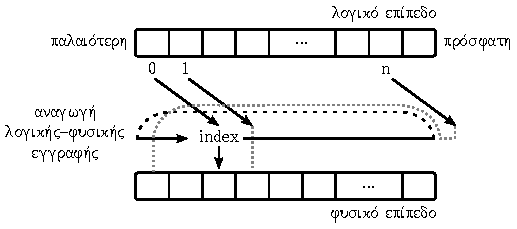
\includegraphics{log_structure}
    \end{center}
\end{figure}


\section{Ώρα συστήματος}
\label{sec:rtc}

Η υλοποίηση περιλαμβάνει τη χρήση ενός ολοκληρωμένου ως ρολόι πραγματικού χρόνου
(\te{Real-Time Clock - RTC}), το DS1307, το οποίο παρέχει ημερομηνία και ώρα
μέχρι δευτερολέπτων, χαρακτηρίζεται από καλή ακρίβεια (απώλεια μερικών
δευτερολέπτων το μήνα), χαμηλή κατανάλωση ισχύος και δυνατότητα διατήρησης της
λειτουργίας του με εφεδρική τροφοδοσία (μέσω μπαταρίας).

Το RTC διαθέτει 7 καταχωρητές για την ημερομηνία\slash{}ώρα και έναν για τη
ρύθμιση του παραγόμενου τετραγωνικού παλμού, ενώ ορισμένα bit ελέγχου βρίσκονται
σε ορισμένες θέσεις των καταχωρητών ημερομηνίας\slash{}ώρας
\parencite[8]{ds1307}. Η ημερομηνία\slash{}ώρα
αναπαριστάται με συμβολισμό BCD (\te{packed Binary-Coded Decimal}) σύμφωνα με
τον οποίο κάθε δεκαδικό ψηφίο αποθηκεύεται σε 4bit \parencite[8]{ds1307}.
Για παράδειγμα, ο αριθμός 12 του δεκαδικού συστήματος αρίθμησης αποκτά δυαδική
αναπαράσταση 0001~0002 αντί της συνήθης 0000~1100.

Κατά την αρχική σύνδεση με τη τροφοδοσία, το ρολόι είναι απενεργοποιημένο, κάτι
που σηματοδοτείται από την ένδειξη CH (\te{Clock Halt}) του καταχωρητή 0x00
\parencite[8]{ds1307}. Η επαναφορά του σε 0 ενεργοποιεί το ρολόι και μπορεί να
πραγματοποιηθεί παράλληλα με την αρχική ενημέρωση της ημερομηνίας\slash{}ώρας.

Η επικοινωνία του RTC με το μικροελεγκτή πραγματοποιείται μέσω διαύλου
I\tsup{2}C (\te{Inter-Integrated Circuit}) σύμφωνα με τον οποίο ο μικροελεγκτής
(\te{master} του διαύλου) αποστέλλει το \te{bit START} ακολουθούμενο από τη
διεύθυνση του RTC (στην προκειμένη, 0x68) και το bit πρόθεσης R\slash\nbar{W}
(βλ. \nameref{subsec:i2c} σ.~\pageref{subsec:i2c}) \parencite[1,10]{ds1307}.

\begin{figure}
    \caption{Παράδειγμα εγγραφής και ανάγνωσης από διεύθυνση του RTC.
    \label{fig:rtc:start-r}}
    \begin{center}
    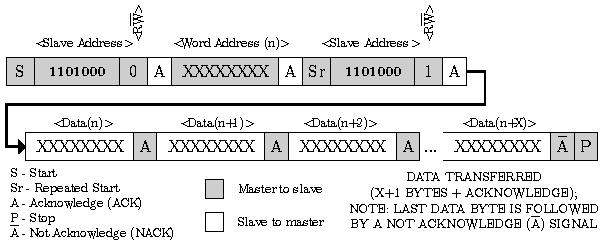
\includegraphics{ds1307_start-r}
    \end{center}
    \fullcite[13]{ds1307:start-r}
\end{figure}

Κατόπιν, ακολουθεί η διεύθυνση του καταχωρητή προς ανάγνωση\slash{}εγγραφή (του
RTC) και το επιθυμητό πλήθος Byte. Σαφώς, παρεμβάλλονται τα \te{bit} ACK μετά
την κάθε επιτυχούσα παραλαβή Byte. Το σχήμα \ref{fig:rtc:start-r} παρουσιάζει
την αποστολή της επιθυμητής διεύθυνσης του RTC (\te{Word Address (n)}), την
επανεκκίνηση της επικοινωνίας (Sr) σε λειτουργία ανάγνωσης και την παραλαβή ενός
πλήθους Byte από το RTC. Σημειώνεται ότι το RTC DS1307 υποστηρίζει ανάγνωση%
\slash{}εγγραφή σε \te{burst mode}, σύμφωνα με την οποία ο εσωτερικός δείκτης
της επιθυμητής διεύθυνσης αυξάνεται αυτόματα με τη διεκπεραίωση κάθε Byte
\parencite[12]{ds1307}.


\subsection{Μνήμη RAM}
\label{subsec:rtc:user-ram}

Το RTC DS1307 διαθέτει κοινόχρηστη μνήμη 56Byte η οποία διατηρεί τα δεδομένα της
ακόμα και όταν το RTC μεταπίπτει στην εφεδρική τροφοδοσία (μπαταρία)
\parencite[1]{ds1307}. Το χαρακτηριστικό αυτό είναι ιδιαίτερα χρήσιμο, καθώς η
μνήμη του μπορεί να χρησιμοποιηθεί για την αποθήκευση ρυθμίσεων της συσκευής που
διατηρούνται μεταξύ διαδοχικών αποσυνδέσεών της από την κύρια τροφοδοσία που,
ωστόσο, είναι εύκολο να αναιρεθούν με την προσωρινή αποσύνδεση της μπαταρίας από
τη συσκευή (προκαλώντας επαναφορά στις εργοστασιακές της ρυθμίσεις) (βλ.
\nameref{subsec:backup-memory} σ.~\pageref{subsec:backup-memory}).

Οι διευθύνσεις της μνήμης έπονται των καταχωρητών (διεύθυνση 0x08) και
εκτείνονται μέχρι την 0x3F \parencite[8]{ds1307}.

%\subsection{Συνδεσμολογία}
% XTAL frequency, ground plane


\section{Ανάθεση εργασιών}
\label{sec:task}

Στο κεφάλαιο του υποσυστήματος κίνησης (σ.~\pageref{ch:motor})
παρουσιάζεται ο υποκείμενος μηχανισμός για τον έλεγχο της κίνησης της κεφαλής
της συσκευής.
Ωστόσο, στο πλαίσιο της υλοποίησης, η χρήση του υποσυστήματος κίνησης είναι
άρρηκτα συνδεδεμένη με την πραγματοποίηση μετρήσεων· η κεφαλή μετακινείται σε
μία
θέση με σκοπό τη δειγματοληψία και καταχώρηση της μέτρησης των αισθητήρων για
εκείνο το σημείο του υλικού. Αυτή η πρόσθετη λειτουργία παρέχεται από ξεχωριστό
τμήμα, τη μονάδα εργασίας (\te{task}).


\subsection{Εργασία δειγματοληψίας}

Η πραγματοποίηση μίας εργασίας για τη δειγματοληψία του μέσου μπορεί να
περιγραφεί από τα ακόλουθα στάδια:
\begin{enumerate}
    \item Μετατόπιση κεφαλής σε νέο ζεύγος συντεταγμένων XY.
    \item Διείσδυση της κεφαλής στο παρακολουθούμενο μέσο.
    \item Λήψη μέτρησης των αισθητήρων και καταχώρησή τους στο Ημερολόγιο
    (σ.~\pageref{sec:log}).
    \item Ανύψωση της κεφαλής.
\end{enumerate}

Δεδομένου ότι η κεφαλή βρίσκεται ανυψωμένη (προεπιλεγμένη θέση κατόπιν
παλιννόστησης) (βλ. σ.~\pageref{subsec:motor:homing}),
τα δύο πρώτα στάδια πραγματοποιούνται αυτόματα από τον
υποκείμενο μηχανισμό. Κατά την ολοκλήρωση της μετατόπισης της κεφαλής
(συμπεριλαμβανομένης και της διείσδυσής στο μέσο), το υποσύστημα κίνησης
ενημερώνει για το συμβάν (μέσω επανάκλησης) το υποσύστημα εργασίας (ή όποιο άλλο
του έχει δηλωθεί).

Στο σημείο αυτό, η μονάδα εργασίας αναλαμβάνει το 3\tsup{ο} στάδιο. Κατόπιν,
προκαλεί την ανύψωση της κεφαλής, η οποία εκτελείται ασύγχρονα (όπως συμβαίνει,
άλλωστε, με κάθε κίνηση της κεφαλής). Η μονάδα εργασίας ειδοποιείται ξανά
όταν η κεφαλή έχει επανατοποθετηθεί στην κορυφαία της θέση. Πλέον, εφόσον
απαιτείται, είναι δυνατό να δρομολογηθεί μία νέα μέτρηση προκαλώντας τη
μετατόπιση της κεφαλής σε νέες συντεταγμένες XYZ με $\text{Z} = 0$, ώστε το
υποσύστημα εργασίας να ειδοποιηθεί όταν η κεφαλή βρίσκεται σε θέση για νέα
δειγματοληψία.

Στο σχήμα \ref{fig:task:samples} παρουσιάζεται πώς το υποσύστημα εργασίας
προκαλεί την αρχική ενεργοποίηση τους υποσυστήματος κίνησης (για τη μετακίνηση
σε νέα θέση) και πώς οι διαδοχικές διεκπεραιώσεις της μετακίνησης της κεφαλής
οδηγούν, σταδιακά, στην ολοκλήρωση του ανατεθειμένου πλήθους μετρήσεων. Η
ενεργοποίηση της εργασίας παραλείπεται το σχήμα, εσκεμμένα, και ο λόγος
περιγράφεται στην \nameref{ssubsec:task:initiate}
(σ.~\pageref{ssubsec:task:initiate}).

\begin{figure}
    \caption{Σταδιακή ολοκλήρωση φόρτου εργασίας μετρήσεων.
    \label{fig:task:samples}}
    \begin{center}
    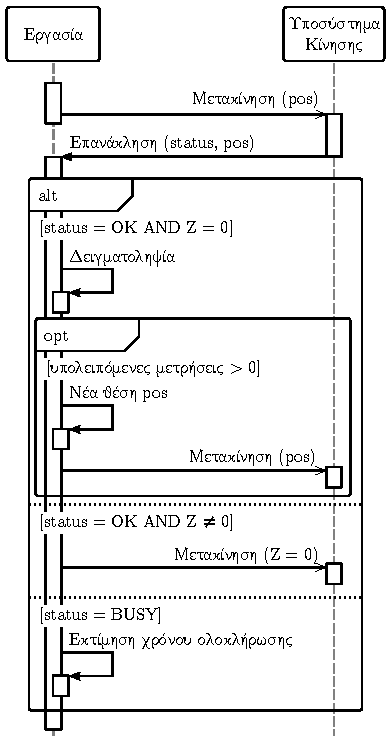
\includegraphics{task_samples}
    \end{center}
\end{figure}

Ένα αναγκαίο στοιχείο για την πραγματοποίηση πολλαπλών μετρήσεων είναι η ύπαρξη
ενός μηχανισμού για την παραγωγή νέων, προς δειγματοληψία, θέσεων. Ένας τέτοιος
μηχανισμός θα μπορούσε να λαμβάνει υπόψη προηγούμενες μετρήσεις ώστε να
προτιμώνται τοποθεσίες που έχουν καιρό να υποστούν εξέταση ή εκείνες στις οποίες
είχαν εντοπιστεί κρίσιμες τιμές. Ωστόσο, στο πλαίσιο της υλοποίησης, ο
μηχανισμός αρκείται στην παραγωγή τυχαίων θέσεων που βασίζονται, ελαφρώς, στην
τρέχουσα ημέρα και ώρα της συσκευής
% \nref : RTC
και στην τρέχουσα θέση της κεφαλής.


\subsubsection{Εκτιμώμενος χρόνος ολοκλήρωσης}

Στο σχήμα \ref{fig:task:samples} γίνεται αναφορά σε εκτίμηση του χρόνου
ολοκλήρωσης η οποία εκτελείται όποτε η επανάκληση αναφέρει ότι το υποσύστημα
κίνησης είναι απασχολημένο (\te{BUSY}). Ο λόγος ύπαρξης του μηχανισμού εκτίμησης
είναι η
παροχή μίας ένδειξης του χρόνου για τον οποίο το υποσύστημα κίνησης, καθώς και
όλες οι λειτουργίες που βασίζονται σε αυτόν, είναι αδύνατο να χρησιμοποιηθούν
έως ότου παρέλθει. Χαρακτηριστική περίπτωση χρήσης του εκτιμώμενου χρόνου είναι
στο πεδίο κεφαλίδας HTTP \te{Retry-After} κατά τις αποκρίσεις με κωδικούς
κατάστασης 202 και 503 (βλ. \nameref{sec:network:impl-resources}
σ.~\pageref{sec:network:impl-resources}).

Όπως αναφέρεται στο Υποσύστημα Κίνησης
(σσ.~\pageref{ssubsec:motor:routing},%
\pageref{ssubsec:motor:common-translation}),
η μετατόπιση της κεφαλής σε νέα θέση πραγματοποιείται σε τρία, το πολύ, στάδια·
κοινή μετατόπιση στο επίπεδο X-Y, υπολειπόμενη μετατόπιση σε άξονα X ή Υ και
μετατόπιση σε άξονα Z ή, εναλλακτικά, πρώτα η μετατόπιση στον άξονα Z και μετά
των άλλων δύο. Πριν την εκκίνηση κάθε σταδίου, και ενώ οι κινητήρες
βρίσκονται σε ηρεμία, αναγγέλλεται από το υποσύστημα κίνησης (μέσω της
επανάκλησης) ο νέος προορισμός και η αλλαγή της κατάστασής του σε \te{BUSY}. Η
πληροφορία αυτή σε συνδυασμό το υπολειπόμενο πλήθος μετρήσεων μπορεί να
χρησιμοποιηθεί για την εκτίμηση της συνολικής διάρκειας της εργασίας.

\begin{figure}
    \caption{Στάδια περάτωσης μίας εργασίας μέτρησης.
    \label{fig:task:estimate-update}}
    Οι στιγμές αναγγελίας \te{BUSY} (βέλη) αποτελούν τα σημεία όπου ανανεώνεται
    η εκτίμηση του χρόνου ολοκλήρωσης. Ο αστερίσκος (*) δηλώνει μία ενδεχόμενη
    πρόσθετη αναγγελία, εφόσον υπολείπεται κίνηση σε έναν εκ των δύο αξόνων X ή
    Y.
    \begin{center}
    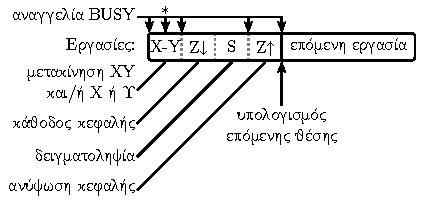
\includegraphics{task_estimate-update}
    \end{center}
\end{figure}

Το σχήμα \ref{fig:task:estimate-update} παρουσιάζει τις συνιστώσες της εργασίας
καθώς και τις στιγμές που αναγγέλλεται η ολοκλήρωση ενός μέρους της μετατόπισης
(σημεία \te{BUSY}). Στο σχήμα, στην περίπτωση της μετατόπισης στο επίπεδο X-Y,
σημειώνεται μία ενδεχόμενη δεύτερη αναγγελία (με αστερίσκο) όταν
πραγματοποιείται ξεχωριστή μετατόπιση σε έναν εκ των δύο αξόνων για το
υπολειπόμενο πλήθος βημάτων. Η λεπτομέρεια αυτή είναι αδιάφορη για τη μονάδα
εργασίας, καθώς αυτό που ενδιαφέρει σε σχέση με το επίπεδο X-Y, είναι η μέγιστη
μετατόπιση μεταξύ των δύο αξόνων.

Όπως αναφέρεται προηγουμένως, η νέα θέση της κεφαλής στο επίπεδο X-Y
υπολογίζεται τη στιγμή ολοκλήρωσης της προηγούμενης εργασίας. Αυτή η σχεδιαστική
επιλογή καθιστά αδύνατο τον ακριβή υπολογισμό του χρόνου ολοκλήρωσης του συνόλου
των εργασιών καθώς οι θέσεις που, τελικά, θα προκύψουν είναι άγνωστες σε
προγενέστερη στιγμή της εκτέλεσης.

Για το λόγο αυτό χρησιμοποιείται ένας αναμενόμενος χρόνος μετατόπισης της
κεφαλής στο επίπεδο X-Y για τις υπολειπόμενες εργασίες ο οποίος, όσο μεγαλύτερο
το πλήθος εργασιών, τόσο μεγαλύτερη απόκλιση από τον πραγματικό χρόνο που
τελικά θα απαιτηθεί. Ωστόσο, καθώς ολοκληρώνονται τα επιμέρους στάδια κάθε
εργασίας και πραγματοποιείται νέα εκτίμηση (σημεία αναγγελίας \te{BUSY}), ο
εκτιμώμενος χρόνος γίνεται ολοένα πιο έγκυρος. Η απόκλιση της εκτίμησης του
χρόνου ολοκλήρωσης της τελευταίας εργασίας κυμαίνεται στα 2, περίπου,
δευτερόλεπτα, μετρική αποδεκτή για τις απαιτήσεις της υλοποίησης.

Η εκτίμηση του χρόνου ολοκλήρωσης του φόρτου εργασίας καθώς και η ώρα κατά την
οποία πραγματοποιήθηκε η εκτίμηση, διατηρούνται. Όποτε προκύπτει ανάγκη για την
επιστροφή του αναμενόμενου χρόνου ολοκλήρωσης ξεκινώντας κάποια δεδομένη χρονική
στιγμή, αρκεί να αφαιρεθεί από εκείνη την ώρα, η ώρα της τελευταίας εκτίμησης
και να συγκριθεί το αποτέλεσμα με την εκτίμηση χρόνου για να διαπιστωθεί πόσος
εκτιμημένος χρόνος έχει παρέλθει.


\subsubsection{Εκκίνηση εργασίας}
\label{ssubsec:task:initiate}

Η δειγματοληψία του μέσου είναι δυνατό να ξεκινήσει με δύο τρόπους· κατόπιν
προτροπής εξωτερικής οντότητας ή από το ίδιο το σύστημα υπό τις κατάλληλες
συνθήκες. Η εκκίνηση εργασιών από εξωτερική οντότητα περιγράφεται στη μέθοδο
\te{POST} του πόρου μετρήσεων του διακομιστή
(σ.~\pageref{ssubsec:network:measurement-post}) και παρέχεται κυρίως για λόγους
εξακρίβωσης λειτουργίας.

Η κύρια πηγή εκκίνησης των κύκλων εργασιών παραμένει το ίδιο το σύστημα.
Για το σκοπό αυτό, κρίνεται
αρκετή η τήρηση της ώρας της πιο πρόσφατης μέτρησης και μίας ένδειξης για το
ελάχιστο επιθυμητό διάστημα μεταξύ διαδοχικών κύκλων εργασίας. Επίσης,
απαιτείται η ύπαρξη ενός ελέγχου για την εξακρίβωση του χρόνου που έχει παρέλθει
από την πλέον πρόσφατη μέτρηση μέχρι τη στιγμή που πραγματοποιείται ο έλεγχος.

Προφανώς, η ημερομηνία της πλέον πρόσφατης μέτρησης τίθεται κατά την
αρχικοποίηση της συσκευής (\te{power-on}) βάσει της τελευταίας καταχωρημένης
εγγραφής του ημερολογίου και ενημερώνεται με κάθε νέα πραγματοποιηθείσα μέτρηση.

Ωστόσο, στην πραγματικότητα, ο μηχανισμός βασίζεται στη χρήση χρονοσφραγίδων που
αντιπροσωπεύουν τα λεπτά που έχουν παρέλθει από την αρχή της ημέρας για κάθε
ημερομηνία. Για την ακρίβεια, επιλέγεται η ημέρα να χωρίζεται σε 240 κβάντα, ενώ
κάθε χρονοσφραγίδα προσδιορίζει κάποια στιγμή της ημέρας ως ένα πλήθος τέτοιων
κβάντων. Όποτε προκύπτει ανάγκη για τον έλεγχο του χρονικού διαστήματος που έχει
παρέλθει μεταξύ πρόσφατης και τρέχουσας ώρας, η τρέχουσα ώρα ανάγεται σε
χρονοσφραγίδα (δηλαδή, σε κβάντα των 6 λεπτών) και συγκρίνεται με τη
χρονοσφραγίδα της μέτρησης (σχήμα \ref{fig:task:interval}).

\begin{figure}
    \caption{Αντιστοίχηση ωρών σε κβάντα και υπολογισμός χρονικού διαστήματος.
    \label{fig:task:interval}}
    Με n συμβολίζεται η κάθε ώρα της ημέρας και κυμαίνεται μεταξύ 0 και 23, ενώ
    για κάθε ώρα ορίζονται 10 κβάντα. Συνολικά, μία μέρα διαθέτει 240 κβάντα.
    \begin{center}
    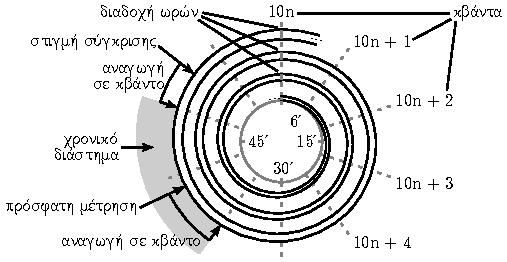
\includegraphics{task_interval}
    \end{center}
\end{figure}

Ο υπολογισμός της χρονοσφραγίδας είναι απλός· οι ώρες μετατρέπονται σε λεπτά και
χωρίζονται σε κβάντα, κατόπιν, προστίθεται η αξία (ευκλείδεια διαίρεση) των
λεπτών σε κβάντα, ως εξής:
\begin{equation}
Q = \frac{60 hrs + min}{q}
\end{equation}
, όπου $q$ η αξία κάθε κβάντου σε λεπτά ($q = 6$).

Ως άμεσο αποτέλεσμα, είναι δυνατή η διάκριση των ωρών με ακρίβεια το πολύ 6
λεπτών. Επιπλέον, η τήρηση μέχρι 240 κβάντων (δηλαδή, μίας ημέρας) συνεπάγεται
ότι οι δύο ημερομηνίες συγκρίνονται μόνο ως προς τις ώρες και τα λεπτά,
αγνοώντας τη διαφορά τους σε ημέρες, μήνες και έτη. Τυπικά, το πρόβλημα αυτό
είναι αμελητέο καθώς η σύγκριση των χρονοσφραγίδων πραγματοποιείται κάθε λίγα
δευτερόλεπτα. Μόνο στην περίπτωση παρατεταμένης διακοπής της τροφοδοσίας του
ρεύματος ενδέχεται να εμφανιστεί κάποια ασυνέχεια με τη μορφή καθυστερημένης
εκκίνησης του επόμενου κύκλου εργασίας που οφείλεται στο ότι η συσκευή αναμένει
να παρέλθει το καθορισμένο πλήθος κβάντων από την τελευταία \emph{ώρα} μέτρησης,
ανεξαρτήτως της ημέρας κατά την οποία πραγματοποιήθηκε.


\subsubsection{Περιοδικός έλεγχος}

Είναι σαφές ότι ο έλεγχος της χρονοσφραγίδας απαιτεί ένα έναυσμα που να προκαλεί
την εκτέλεσή του. Επίσης, θα πρέπει να είναι ικανό να αφυπνίζει τη μονάδα
επεξεργασίας από λειτουργία χαμηλής κατανάλωσης που αυτή τίθεται όσο αναμένει
κάποια νέα εργασία. Σύμφωνα με το εγχειρίδιο της \textcite[38]{atmel13}, ο
χρονομετρητής WDT (\te{Watchdog Timer}) μπορεί να χρησιμοποιηθεί για την
αφύπνιση της MCU από οποιαδήποτε λειτουργία χαμηλής κατανάλωσης.

Ο χρονομετρητής WDT χρησιμοποιεί παλμούς ανεξάρτητου ταλαντωτή και ρυθμίζεται
για περιοδική ενεργοποίηση (μέσα από ένα εύρος πιθανών περιόδων) κατά την οποία
προκαλεί διακοπή ή ακόμα και επανεκκίνηση του μικροελεγκτή (\te{reset})
\parencite[50]{atmel13}. Το δεύτερο είναι ιδιαίτερα σημαντικό για την αποφυγή
ατερμόνων βρόχων αλλά απαιτεί την, από λογισμικού, επανέναρξη του μετρητή πριν
την πρόκληση της επανεκκίνησης \parencite[50]{atmel13}.

Στο πλαίσιο της υλοποίησης, ο WDT ρυθμίζεται μόνο για την αναγγελία διακοπής, η
οποία είτε αφυπνίζει την MCU και εκτελεί τη ρουτίνα εξυπηρέτησης της, είτε
αναμένει την ολοκλήρωση κάποιας άλλης ρουτίνας (για παράδειγμα, την απόκριση σε
κάποιο εισερχόμενο αίτημα HTTP) πριν εκτελεστεί η ίδια για την εκκίνηση του
επόμενου κύκλου εργασίας, εφόσον απαιτείται. Σημειώνεται ότι ο επιλεγμένος
μικροελεγκτής (ATmega328P), υποστηρίζει περιόδους από 16ms μέχρι 8s
\parencite[55]{atmel13}.


\subsection{Μέτρηση θερμοκρασίας}
\label{subsec:ds18b20}

%Συνολικά, απαιτούνται τρία αισθητήρια όργανα για την κάλυψη των βασικών αναγκών
%του συστήματος· θερμοκρασία, υγρασία και οξύτητα.
Στο παρόν στάδιο της υλοποίησης, μόνο η μελέτη και διασύνδεση με τον αισθητήρα
θερμοκρασίας υλοποιείται.
Η μέτρηση της θερμοκρασίας αναλαμβάνεται από ψηφιακό θερμόμετρο, το ολοκληρωμένο
DS18B20, το οποίο βρίσκεται ενσωματωμένο σε στεγανό σωληνάριο και προσαρτημένο
στην κινητή κεφαλή της συσκευής ώστε καθώς αυτή κινείται να επιτρέπεται η
μεταφορά του γύρω και εντός του παρακολουθούμενου υλικού. Το επιλεγμένο
ολοκληρωμένο χαρακτηρίζεται από ακρίβεια $\pm0.5^\circ$C σε θερμοκρασία
λειτουργίας $-55$ έως $+125^\circ$C, διασύνδεση 1-Wire (βλ. σ.~%
\pageref{subsec:1-wire}) με δυνατότητα τροφοδοσίας από τη (μοναδική) γραμμή του
διαύλου με ρυθμιζόμενη ακρίβεια από 9 έως 12bit \parencite[1]{ds18b20}.

\begin{figure}
    \caption{Πτητική μνήμη (\te{scratchpad}) και μνήμη EEPROM του DS18B20.
    \label{fig:ds18b20:memories}}
    \begin{center}
    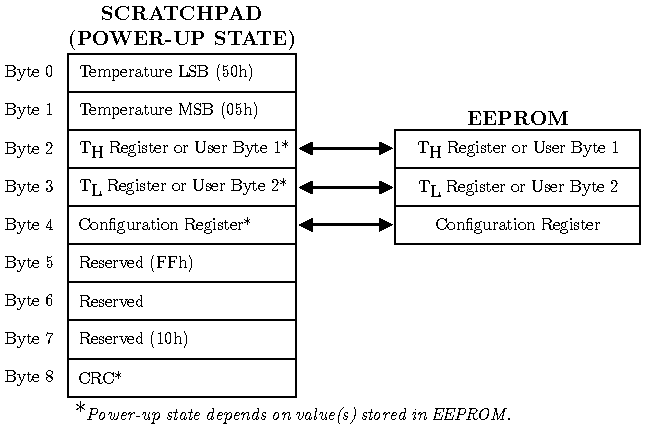
\includegraphics{ds18b20_memories}
    \end{center}
    Βασισμένο \fullcite[7]{ds18b20:memories}
\end{figure}


\subsubsection{Καταχωρητές DS18B20}
\label{ssubsec:ds18b20:registers}

Η μνήμη του αποτελείται από 9Byte με πλέον σημαντικά, για τις ανάγκες της
υλοποίησης, τα δύο πρώτα, στα οποία εναποτίθεται η μέτρηση της θερμοκρασίας.
Ακολουθούν δύο καταχωρητές που προσδιορίζουν δύο όρια θερμοκρασιών τα οποία αν
ξεπεραστούν από κάποια μέτρηση, θέτουν σχετική ένδειξη στην εσωτερική κατάσταση
του ολοκληρωμένου, η οποία μπορεί να χρησιμοποιηθεί για τη συμμετοχή στη
διαδικασία επιλογής \te{slave} συσκευής, μόνο εκείνων των ολοκληρωμένων που
χρήζουν άμεσης ανάγκης \parencite[4--5]{ds18b20}. Προφανώς, συγκρίνεται μόνο το
ακέραιο τμήμα της θερμοκρασίας με την τιμή των καταχωρητών καθώς οι καταχωρητές
είναι του 1Byte ο καθένας (βλ. και σχήμα \ref{fig:ds18b20:t-format}). Η σχετική
εντολή ROM ονομάζεται \te{ALARM SEARCH}. Εναλλακτικά, μπορούν να χρησιμοποιηθούν
για την αποθήκευση δεδομένων της συσκευής που, σε συνδυασμό με την εντολή
\te{COPY SCRATCHPAD} (βλ. παρακάτω), διατηρούνται μεταξύ διαδοχικών αποσυνδέσεων
της συσκευής από την τροφοδοσία.

Ο καταχωρητής στη διεύθυνση 4 καθορίζει την ακρίβεια και, συνεπώς το χρόνο που
απαιτεί κάθε μέτρηση \parencite[4,8]{ds18b20}. Υποστηρίζεται ακρίβεια των 12 έως
9bit, με κάθε μικρότερη να απορρίπτει ένα μέρος του κλάσματος της μέτρησης.

Τα Byte 5 έως 7 χρησιμοποιούνται για τις ανάγκες του ολοκληρωμένου, ενώ στο Byte
8 υπολογίζεται το αποτέλεσμα του πολυωνύμου για την επιβεβαίωση της εγκυρότητας
των δεδομένων κατά την ανάγνωσή τους από το \te{master}.

Η μορφή με την οποία αποθηκεύεται η θερμοκρασία στους δύο πρώτους καταχωρητές
παρουσιάζεται στο σχήμα \ref{fig:ds18b20:t-format}. Η θερμοκρασία αποθηκεύεται
με πρόσημο ως συμπλήρωμα του 2 \parencite[3]{ds18b20}. Στο πλαίσιο της
υλοποίησης, αυτοί είναι οι μοναδικοί καταχωρητές του DS18B20 που αξιοποιούνται.

\begin{figure}
    \caption{Μορφή θερμοκρασίας στους καταχωρητές 0 και 1 του DS18B20.
    \label{fig:ds18b20:t-format}}
    \begin{center}
    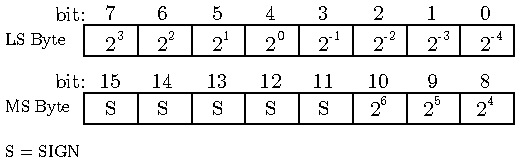
\includegraphics{ds18b20_t-format}
    \end{center}
    Βασισμένο \fullcite[4]{ds18b20:t-format}
\end{figure}

\subsubsection{Υποστηριζόμενες εντολές}
\label{ssubsec:ds18b20:commands}

Στην ενότητα \nameref{subsec:1-wire} (σ.~\pageref{subsec:1-wire}) περιγράφεται η
έννοια της συναλλαγής κατά την οποία πραγματοποιείται αρχικοποίηση, ακολουθεί η
επιλογή μία συσκευής \te{slave} μέσω εντολών ROM και, τελικά, αποστέλλεται η
εντολή λειτουργίας (\te{Function command}) που είναι επιθυμητό να εκτελεστεί.
Στην περίπτωση του DS18B20, οι υποστηριζόμενες εντολές λειτουργίας είναι οι
ακόλουθες:
\begin{description}
    \item[CONVERT T [0x44{]}] Προκαλεί την λήψη μίας νέας μέτρησης. Σε περίπτωση
    που η τροφοδοσία του ολοκληρωμένου είναι ανεξάρτητη από τη γραμμή του
    διαύλου, η ολοκλήρωση σηματοδοτείται από την απελευθέρωση της γραμμής από
    το DS18B20 και την επαναφορά του σε λογικό 1 από τον αντιστάτη \te{pull-up}
    \parencite[11]{ds18b20}. Σε αντίθετη περίπτωση, ο μικροελεγκτής είναι
    υποχρεωμένος να αποφασίσει πόσο χρόνο να αναμείνει ώστε να ολοκληρωθεί η
    μετατροπή, με μέγιστο 750ms για ακρίβεια 12bit \parencite[8,11]{ds18b20}.

    \item[WRITE SCRATCHPAD [0x4E{]}] Επιτρέπει την αποστολή τριών Byte που
    εναποτίθενται στις διευθύνσεις 2, 3 και 4 της πτητικής μνήμης του
    ολοκληρωμένου (καταχωρητές T\tsub{H}, T\tsub{L} και ρυθμίσεων)
    \parencite[11]{ds18b20}.

    \item[READ SCRATCHPAD [0xBE{]}] Επιτρέπει την πλήρη ή μερική ανάγνωση της
    πτητικής μνήμης του ολοκληρωμένου ξεκινώντας από το λιγότερο σημαντικό
    \te{bit} του Byte 0, διαδοχικά εκτεινόμενη προς στις επόμενες θέσεις
    \parencite[11]{ds18b20}.

    \item[COPY SCRATCHPAD [0x48{]}] Μεταφέρει τα Byte T\tsub{H}, T\tsub{L} και
    ρυθμίσεων (Byte 2, 3 και 4, αντιστοίχως) από την πτητική μνήμη του DS18B20
    στη μνήμη EEPROM ώστε να διατηρούνται μεταξύ διαδοχικών αποσυνδέσεων του
    ολοκληρωμένου \parencite[12]{ds18b20}.

    \item[RECALL E\protect\tsup{2} [0xB8{]}] Επαναφέρει τα Byte 2, 3 και 4 από
    τη μνήμη EEPROM στην πτητική μνήμη του DS18B20 \parencite[12]{ds18b20}.

    \item[READ POWER SUPPLY [0xB4{]}] Επιτρέπει στο \te{master} να αναγνωρίσει
    εάν το ολοκληρωμένο τροφοδοτείται μέσω του ακροδέκτη V\tsub{CC} ή εάν
    βασίζεται στη γραμμή του διαύλου \parencite[12]{ds18b20}.
\end{description}

\begin{figure}
    \caption{Συναλλαγές 1-Wire για τη δειγματοληψία της θερμοκρασίας.
    Στην υλοποίηση, χρησιμοποιείται μόνο το DS18B20 ως \te{slave} συσκευή με
    αποτέλεσμα να μην απαιτείται η ρητή αναγγελία του αναγνωριστικού του, και
    για αυτό χρησιμοποιείται η εντολή SKIP ROM. Με DQ συμβολίζεται η κατάσταση
    της γραμμής του διαύλου 1-Wire, ενώ ο τερματικός Παλμός \te{Reset} θα
    μπορούσε, κάλλιστα, να ανήκει σε επόμενο ζεύγος παλμών αρχικοποίησης
    (βλ. σ.~\pageref{ssubsec:1-wire:initialisation}).
    \label{fig:ds18b20:sample}}
    \begin{center}
    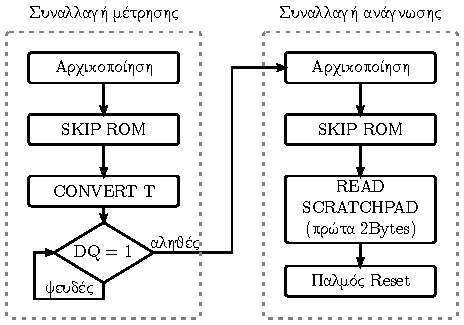
\includegraphics{ds18b20_sample}
    \end{center}
\end{figure}

Στο πλαίσιο της υλοποίησης, οι εντολές που χρησιμοποιούνται είναι οι \te{CONVERT
T} και \te{READ SCRATCHPAD}. Μία τυπική επικοινωνία μεταξύ του μικροελεγκτή και
του DS18B20 απεικονίζεται στο σχήμα \ref{fig:ds18b20:sample} κατά την οποία
πραγματοποιούνται δύο συναλλαγές, μία για την εκκίνηση της μέτρησης και μία για
την ανάγνωση της μνήμης και, για την ακρίβεια, των δύο πρώτων καταχωρητών που
αντιστοιχούν στη μέτρηση. Αυτό είναι δυνατό να επιτευχθεί αποστέλλοντας τον
παλμό \te{Reset} αμέσως μετά την ανάγνωση του δεύτερου \te{Byte}.

Όπως παρουσιάζεται στο σχήμα, η επιλογή του DS18B20 γίνεται μέσω της εντολής
\te{SKIP} ROM η οποία, στην πραγματικότητα, παραλείπει την αναγγελία
αναγνωριστικού και μεταβαίνει, απευθείας, στην αποστολή εντολής λειτουργίας
(\te{Function command}). Η συγκεκριμένη τακτική μπορεί να χρησιμοποιηθεί υπό την
προϋπόθεση ότι το DS18B20 είναι το μοναδικό ολοκληρωμένο που συνδέεται στο
δίαυλο 1-Wire, κάτι που ισχύει για την υλοποίηση. Σε αντίθετη περίπτωση, η
επιλογή περισσότερων ολοκληρωμένων θα προκαλούσε σύγκρουση κατά την ανάγνωση της
μέτρησης όπου ταυτόχρονα θα επιχειρούσαν να αναγγείλουν τα \te{bit} τους.

Τέλος, αναφέρεται ότι κατόπιν υποβολής της εντολής μέτρησης της θερμοκρασίας, ο
μικροελεγκτής αναμένει την απελευθέρωση (και επαναφορά σε λογικό 1) της γραμμής
του διαύλου από το DS18B20 προκειμένου να προβεί στη συναλλαγή της ανάγνωσης. Η
δυνατότητα αναγγελίας της ολοκλήρωσης με αυτόν τον τρόπο είναι διαθέσιμη, όπως
αναφέρεται παραπάνω, μόνο στην περίπτωση που το DS18B20 τροφοδοτείται μέσω του
ακροδέκτη V\tsub{CC} και όχι μέσω της ίδιας της γραμμής του διαύλου.

Στο πλαίσιο της υλοποίησης επιλέγεται η χρήση του ακροδέκτη V\tsub{CC} για την
τροφοδοσία του DS18B20 για δύο λόγους.
Καταρχήν, για τη τροφοδοσία του ολοκληρωμένου μέσω της γραμμής, η
\textcite[5]{ds18b20} συνιστά τη χρήση ενός ισχυρού στοιχείου για την επαναφορά
της (όπως MOSFET) και όχι μόνο ενός αντιστάτη καθώς κατά την μέτρηση της
θερμοκρασίας, η απότομη αύξηση κατανάλωσης έντασης ρεύματος μπορεί να προκαλέσει
πτώση στην τάση της γραμμής με αποτέλεσμα η εργασία να μην ολοκληρωθεί επιτυχώς.
Με τη σειρά του, η μέθοδος αυτή απαιτεί ένα επιπλέον τρανζίστορ καθώς και την
απόδοση ενός επιπρόσθετου ακροδέκτη του μικροελεγκτή για το σκοπό.

Ο δεύτερος λόγος σχετίζεται με τη μορφή του αισθητήριου οργάνου. Το προϊόν που
χρησιμοποιείται διαθέτει ένα DS18B20 ενσωματωμένο στο ένα άκρο ενός στεγανού
σωληναρίου με τρεις απολήξεις σύνδεσης στο άλλο· V\tsub{CC}, GND και DQ.
Επομένως, ήδη υπάρχει αγωγός για τη σύνδεση του ακροδέκτη V\tsub{CC} με την
τροφοδοσία με αποτέλεσμα η χρήση της γραμμής DQ για την τροφοδοσία να φαντάζει
άσκοπη.


\section{Δίαυλοι επικοινωνίας ολοκληρωμένων}
\label{sec:buses}

Στο πλαίσιο της υλοποίησης, γίνεται χρήση των ακόλουθων διαύλων για την
επικοινωνία του μικροελεγκτή με επιλεγμένα ολοκληρωμένα κυκλώματα:
\begin{description}
    \item[1-Wire] της \te{Dallas Semiconductor}, δίαυλος ασύγχρονης
    ημιαμφίδρομης επικοινωνίας που χρησιμοποιεί μόνο έναν αγωγό (σήμα)
    διασύνδεσης. Χρησιμοποιείται για την επικοινωνία με τον αισθητήρα
    θερμοκρασίας DS18B20. Εφόσον ο μικροελεγκτής αδυνατεί να το υποστηρίξει
    εγγενώς, η υλοποίηση του διαύλου γίνεται εξολοκλήρου σε λογισμικό
    (\te{bit-banging}).

    \item[I\protect\tsup{2}C] της Phillips, δίαυλος σύγχρονης ημιαμφίδρομης
    επικοινωνίας που χρησιμοποιεί δύο αγωγούς σύνδεσης· ένα για συγχρονισμό και
    έναν για δεδομένα. Χρησιμοποιείται για την επικοινωνία με το ρολόι
    πραγματικού χρόνου (RTC) DS1307. Το λογισμικό οδήγησης αξιοποιεί το
    υποκείμενο, και συμβατό, κύκλωμα TWI (\te{Two-Wire Interface}) του
    μικροελεγκτή.

    \item[SPI] ονομασμένο από τη Motorola, δίαυλος σύγχρονης αμφίδρομης
    επικοινωνίας που χρησιμοποιεί τρεις αγωγούς επικοινωνίας -- ρολόι, δεδομένα
    \te{Master} και δεδομένα \te{Slave} -- καθώς και επιπρόσθετη γραμμή επιλογής
    (\nbar{CS}) του εκάστοτε ολοκληρωμένου. Χρησιμοποιείται για την επικοινωνία
    με το ολοκληρωμένο δικτύωσης W5100 και της εξωτερικής μνήμης Flash. Το
    λογισμικό οδήγησης κάθε ολοκληρωμένου αξιοποιεί το υποκείμενο κύκλωμα SPI
    του μικροελεγκτή.
\end{description}

\subsection{Δίαυλος 1-Wire}
\label{subsec:1-wire}

Ο δίαυλος 1-Wire δημιουργήθηκε από την Dallas Semiconductor και για τη
διασύνδεση των συσκευών χρησιμοποιείται μία μόνο γραμμή, η οποία μπορεί να
χρησιμοποιηθεί, υπό περιπτώσεις, και για την τροφοδοσία των συσκευών
επιπροσθέτως της ανταλλαγής δεδομένων \parencite[1]{atmel04}. Η επικοινωνία
είναι ημιαμφίδρομη, ενώ για την αποστολή κάθε \te{bit}, ανεξαρτήτως κατεύθυνσης,
χρησιμοποιούνται χρονοθυρίδες οι οποίες δημιουργούνται από το μοναδικό
\te{master} του διαύλου \parencites[2]{atmel04}[15]{ds18b20}.

\begin{figure}
    \caption{Χρονοθυρίδες εγγραφής και ανάγνωσης στο δίαυλο 1-Wire.
    \label{fig:1-wire:time-slot}}
    \begin{center}
    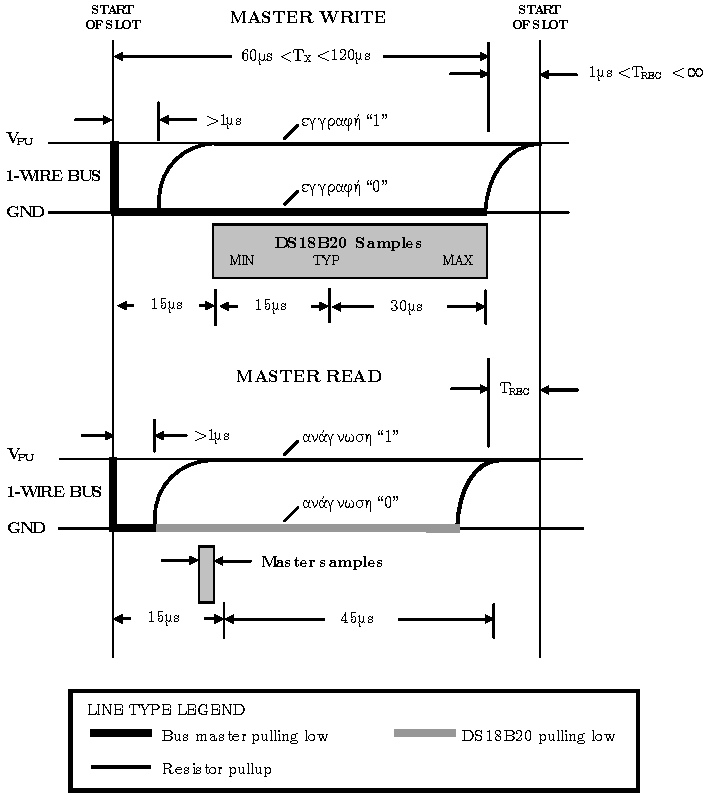
\includegraphics{1-wire_time-slot}
    \end{center}
    Βασισμένο \fullcite[16]{ds18b20:time-slot}
\end{figure}


\subsubsection{Εγγραφή}

Η μορφή των χρονοθυρίδων εμφανίζεται στο σχήμα \ref{fig:1-wire:time-slot}. Σε
περίπτωση εγγραφής ενός \te{bit}, ο \te{master} θέτει τη γραμμή σε λογικό 0 για
1 έως 15μs και, κατόπιν, είτε τη διατηρεί σε αυτήν την κατάσταση αναγγέλλοντας,
με αυτόν τον τρόπο, \te{bit} 0, είτε τίθεται σε κατάσταση υψηλής εμπέδωσης, ώστε
ο αντιστάτης \te{pull-up} να επαναφέρει τη γραμμή σε λογικό 1
\parencite[2]{atmel04}.


\subsubsection{Ανάγνωση}

Για την ανάγνωση ενός \te{bit}, ο \te{master} θέτει τη γραμμή σε λογικό 0
τουλάχιστον για 1μs και, κατόπιν, τίθεται σε κατάσταση υψηλής εμπέδωσης,
δίνοντας τη δυνατότητα στο \te{slave} να αναγγείλει το \te{bit}, ο οποίος, με τη
σειρά του, είτε θέτει τη γραμμή σε λογικό 0, είτε παραμένει σε κατάσταση υψηλής
εμπέδωσης \parencite[2]{atmel04}. Ο \te{master} ελέγχει την κατάσταση της
γραμμής εντός 15μs από την αρχή της χρονοθυρίδας \parencite[17]{ds18b20}
προκειμένου να ανάγει το \te{bit} του \te{slave}.

Είναι εμφανές ότι η ανάγνωση είναι παρόμοια με την εγγραφή \te{bit} τιμής 1·
στην πραγματικότητα, αυτό που διαφοροποιείται είναι η εσωτερική κατάσταση του
\te{slave} που καθορίζει εάν πρόκειται να λάβει ή να εγγράψει κάποιο \te{bit},
όπως, για παράδειγμα, εάν έχει προηγουμένως αποσταλεί εντολή ανάγνωσης κάποιας
διεύθυνσης της μνήμης του.
% \nref : εντολή ανάγνωση μνήμης
Όπως συνιστάται στο εγχειρίδιο της \textcite[17]{ds18b20} και όπως γίνεται ορατό
και στο σχήμα, ο χρόνος κατά τον οποίο η γραμμή παραμένει σε λογικό 0 ως
επενέργεια του \te{master} είναι όσο το δυνατό μικρότερος, ενώ η ανάγνωσή της
γίνεται όσο το δυνατό κοντινότερα στη λήξη του διαστήματος των 15μs. Με αυτόν
τον τρόπο, μειώνεται σημαντικά η πιθανότητα εσφαλμένης ανάγνωσης που οφείλεται
σε μη σταθεροποιημένο σήμα.

Όλες οι χρονοθυρίδες, ανεξαρτήτως εάν πρόκειται για εγγραφή ή ανάγνωση, διαρκούν
από 60 έως 120μs και ακολουθούνται από 1μs, τουλάχιστον, χρόνο ανάκτησης
(T\tsub{REC}) κατά τον οποίο η γραμμή αφήνεται ελεύθερη
\parencites[15--16]{ds18b20}[2]{atmel04}.


\subsubsection{Παλμοί αρχικοποίησης}
\label{ssubsec:1-wire:initialisation}

Η έναρξη της επικοινωνίας μεταξύ \te{master} και \te{slave} γίνεται με την
αποστολή ενός παλμού \te{Reset} από το \te{master} και την απόκριση
του\slash{}των \te{slave} με παλμό \te{Presence} \parencite[15]{ds18b20}. Ο
παλμός \te{Reset} θέτει τη γραμμή σε λογικό 0 τουλάχιστον για 480μs (διάστημα 8
φορές μεγαλύτερο από τις χρονοθυρίδες ανάγνωσης\slash{}εγγραφής), κατόπιν η
γραμμή απελευθερώνεται και εφόσον, εντός 60μs από τη στιγμή εκείνη, η γραμμή
βρίσκεται σε λογικό 0, τότε υπάρχει τουλάχιστον μία συνδεδεμένη \te{slave}
συσκευή στο δίαυλο (παλμός \te{Presence}) \parencite[3]{atmel04}.


\subsubsection{Συναλλαγές}

\begin{figure}
    \caption{Κύκλος συναλλαγής στο δίαυλο 1-Wire.
    \label{fig:1-wire:transaction}}
    Όλες οι συναλλαγές ξεκινούν με τους παλμούς αρχικοποίησης και ακολουθεί η
    επιλογή της επιθυμητής \te{slave} συσκευής και η αποστολή εντολής προς
    αυτήν. Το ακριβές σύνολο εντολών λειτουργίας (\te{Function Command})
    εξαρτάται από την οικογένεια της εκάστοτε συσκευής (για παράδειγμα, λήψη
    θερμοκρασίας από αισθητήρα θερμοκρασίας).
    \begin{center}
    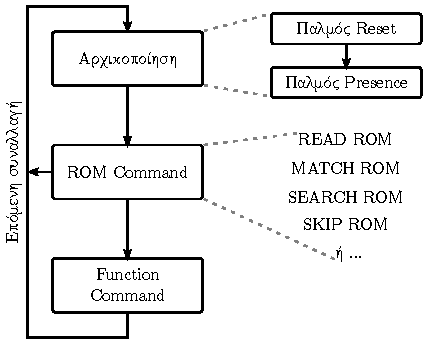
\includegraphics{1-wire_transaction}
    \end{center}
\end{figure}

Στο δίαυλο 1-Wire, εκτός από τους παλμούς αρχικοποίησης και των χρονοθυρίδων
ανάγνωσης\slash{}εγγραφής, ορίζονται ακολουθίες εντολών (δηλαδή, ανταλλαγή
συγκεκριμένων τιμών Byte), αναφερόμενες ως συναλλαγές, για την επίτευξη
οποιασδήποτε λειτουργίας \parencite[10]{ds18b20}. Το σχήμα
\ref{fig:1-wire:transaction} παρουσιάζει τις εργασίες μίας συναλλαγής.
Η αρχικοποίηση έχει περιγραφεί, ενώ οι εντολές λειτουργίας
(\te{Function Command}) εξαρτώνται από τα εκάστοτε είδη των συνδεδεμένων
συσκευών.

\paragraph{Εντολές ROM}%
Ο λόγος ύπαρξης των εντολών ROM αιτιολογείται από την ανάγκη για τον εντοπισμό
και επιλογή μίας συσκευής \te{slave} εκ του συνόλου των συνδεδεμένων στο δίαυλο.
Προκειμένου να είναι αυτό δυνατό, αποδίδεται σε κάθε συσκευή ένα μοναδικό
αναγνωριστικό των 64bit το οποίο περιέχει έναν κωδικό οικογενείας της συσκευής
των 8bit, ένα σειριακό αριθμό των 48bit και κωδικό CRC (\te{Cyclic Redundancy
Check}) των 8bit βάσει των προηγούμενων \te{Byte} \parencite[6]{ds18b20}.
Οι κοινώς υποστηριζόμενες εντολές \te{ROM} είναι οι ακόλουθες:
\begin{description}
    \item[READ ROM [0x33{]}] Επιτρέπει την απευθείας ανάγνωση του
    αναγνωριστικού της μοναδικής \te{slave} συσκευή του διαύλου (δεδομένου ότι
    είναι μόνο μία).

    \item[MATCH ROM [0x55{]}] Για την αναγγελία του επιθυμητού αναγνωριστικού
    των 64bit από το \te{master} και την απόκριση μόνο από το \te{slave} που τον
    διαθέτει. Το συγκεκριμένο μπορεί να χρησιμοποιηθεί εάν, για παράδειγμα,
    είναι, εκ των προτέρων, καταχωρημένα όλα τα πιθανά αναγνωριστικά.

    \item[SEARCH ROM [0xF0{]}] Χρησιμοποιείται για την ανάγνωση των
    αναγνωριστικών των συνδεδεμένων συσκευών, ένα προς ένα, εφόσον τα ακριβή
    στοιχεία τους είναι άγνωστα κατά την εκκίνηση του συστήματος.

    \item[SKIP ROM [0xCC{]}] Παράληψη της επιλογής κάποιας συγκεκριμένης
    συσκευής επειδή πρόκειται να δοθεί η ίδια εντολή σε όλες τις συσκευές ή
    επειδή είναι γνωστό ότι μόνο μία είναι συνδεδεμένη.
\end{description}


\subsubsection{ATmega328P και 1-Wire}

Στο μικροελεγκτή ATmega328P, ο δίαυλος 1-Wire είναι δυνατό να υποστηριχθεί εξ
ολοκλήρου μέσω λογισμικού ή εν μέρει σε λογισμικό και εν μέρει σε υλικό (για
παράδειγμα, USART), χωρίς, ωστόσο, να υπάρχει εγγενώς κάποιο κύκλωμα ειδικά για
αυτόν τον σκοπό \parencite[3]{atmel04}. Στο πλαίσιο της υλοποίησης, επιλέγεται η
πρώτη προσέγγιση (εξ ολοκλήρου σε λογισμικό).

Επιπλέον, δεδομένου ότι χρησιμοποιείται μόνο μία συσκευή (αισθητήρας
θερμοκρασίας), επιλέγεται η μη υλοποίηση της διαδικασίας αναζήτησης \te{slave}
συσκευής (\te{Search ROM}), καθώς η μία που χρησιμοποιείται είναι, εξαρχής,
γνωστή.
% \nref : DS18B20


\subsection{Δίαυλος I\protect\tsup{2}C (TWI)}
\label{subsec:i2c}

%Ο δίαυλος I\tsup{2}C σχεδιάστηκε το 1982 από τη \te{Phillips Semiconductor} με
%αρχικό σκοπό

Βασικά χαρακτηριστικά του διαύλου είναι η διασύνδεση των συσκευών με δύο
γραμμές, τις SDA (\te{Serial DAta}) και SCL (\te{Serial CLock}), τη δυνατότητα
οποιασδήποτε συσκευής να ξεκινήσει την επικοινωνία με κάποια άλλη
(\te{multi-master}) επιλέγοντάς την μέσω μοναδικής διεύθυνσης που διαθέτουν
όλες με συχνότητα του ρολογιού που αναγνωρίζεται από τις ίδιες τις συσκευές
(δεδομένου ότι είναι εντός των επιτρεπτών τους ορίων), χωρίς να απαιτείται
προηγούμενη ρύθμιση κάθε συσκευής ξεχωριστά \parencite[3--4,6]{nxp14}.

Σύμφωνα με την \textcite[6]{nxp14}, προκειμένου κάποια συσκευή να επικοινωνήσει
με κάποια άλλη, απαιτείται πρώτα να αποκτήσει τον έλεγχο του διαύλου (να γίνει
\te{master}). Κατόπιν, αποστέλλει τη διεύθυνση του επιθυμητού \te{slave} (7bit)
ακολουθούμενο από το bit πρόθεσης (λογικό 1 συνεπάγεται ανάγνωση από το
\te{slave}) και λαμβάνει ένα bit επιβεβαίωσης (ACK) από το \te{slave}, σε
περίπτωση επιτυχίας ενώ στη συνέχεια ακολουθούν τα \te{Byte} καθένα συνοδευόμενο
από bit επιβεβαίωσης ή μη \parencite[10,13]{nxp14}.

Σε κατάσταση αδράνειας του διαύλου, οι γραμμές SDA και SCL ηρεμούν σε λογικό 1
μέσω αντιστατών pull-up (αντίστασης, συνήθως, μεταξύ 2--10kΩ) ενώ όλες οι
συνδεδεμένες συσκευές βρίσκονται σε κατάσταση υψηλής εμπέδωσης
\parencites[13]{phillips03}[8]{nxp14}. Σε τυπική λειτουργία, η γραμμή SDA
τίθεται (προετοιμάζεται) όταν η γραμμή SCL βρίσκεται σε λογικό 0. Τη στιγμή που
η SCL ανέρχεται, η SDA θεωρείται ότι έχει σταθεροποιηθεί και οι συνδεδεμένες
συσκευές διαβάζουν την τιμή της. Κατόπιν, η SCL επανέρχεται σε λογικό 0 ώστε η
SDA να τεθεί εκ νέου \parencite[9]{nxp14}.

Επιπλέον, ορίζονται δύο ειδικές περιπτώσεις που χρησιμοποιούνται για την
εκκίνηση και τον τερματισμό της επικοινωνίας από το \te{master} -- η αποστολή
των bit \te{START} και \te{STOP} -- τα οποία αποτελούν τη μεταβολή της SDA σε
λογικό 0 και 1, αντιστοίχως, ενώ η γραμμή SCL βρίσκεται σε λογικό 1
\parencite[9]{nxp14}. Μία υποπερίπτωση αυτών, είναι η αποστολή bit \te{START}
από το \te{master} του διαύλου ώστε να πραγματοποιήσει νέα επικοινωνία (είτε με
την ίδια είτε με άλλη συσκευή) χωρίς να απελευθερώσει το δίαυλο πρώτα το δίαυλο
\parencite[13]{nxp14}. Το bit αυτό αποκαλείται Sr (\te{Repeated Start}) και
είναι ισοδύναμο του bit \te{START} με την εξαίρεση ότι στην περίπτωση που ο
\te{master} λαμβάνει από το \te{slave} πρέπει να αποκριθεί με NACK προτού
αποστείλει το bit Sr \parencite[13--14]{nxp14}.

Ο δίαυλος I\tsup{2}C υποστηρίζει, επίσης, μηχανισμούς διαιτησίας
(\te{arbitration}) και αναγνώρισης συγκρούσεων (\te{collision detection}) που
αξιοποιούνται σε υλοποιήσεις πολλαπλών συσκευών που γίνονται \te{master} του
διαύλου. Στην περίπτωση αυτής της υλοποίησης, \te{master} του διαύλου μπορεί να
είναι μόνο ο μικροελεγκτής και, συνεπώς, αποφεύγεται η περαιτέρω ανάλυσή τους.


%\subsubsection{Two-Wire Interface (TWI)}

Ο μικροελεγκτής της υλοποίησης (ATmega328P) διαθέτει κύκλωμα συμβατό με το
I\tsup{2}C της Phillips υπό το όνομα TWI (\te{Two-Wire Interface}) και δια μέσω
αυτού πραγματοποιείται η διασύνδεσή του με το ολοκληρωμένο
\parencite[209]{atmel13}.

\subsection{Δίαυλος SPI}
\label{subsec:spi}

Η διασύνδεση των συσκευών σε δίαυλο SPI (\te{Serial Peripheral Interface})
γίνεται μέσω τριών, κοινών για όλες τις συσκευές, γραμμών για την ανταλλαγή των
δεδομένων -- SCK (\te{Serial Clock}), MOSI (\te{Master-Out Slave-In}), MISO
(\te{Master-In Slave-Out}) -- και επιπρόσθετων γραμμών για την επιλογή κάθε
\te{slave} συσκευής (\nbar{SS} -- \te{Slave Select})
\parencite[15,24]{motorola04}. Η \te{master} συσκευή είναι υπεύθυνη για την
επιλογή της επιθυμητής, για επικοινωνία, \te{slave} συσκευής καθώς και για την
παραγωγή του ρολογιού, ενώ τα δεδομένα αποστέλλονται ταυτόχρονα και προς τις δύο
κατευθύνσεις \parencite[26--27]{motorola04}.

Στο σχήμα \ref{fig:spi:cpha-0} παρουσιάζονται τα σήματα επικοινωνίας μέσω του
διαύλου SPI. Ο δίαυλος ρυθμίζεται για τη χρήση είτε λογικού 1 είτε 0 ως ενεργό
\te{bit} των παλμών ρολογιού (πολικότητα -- \te{polarity}) καθώς και σε ποια
παρυφή των παλμών του ρολογιού πραγματοποιείται η δειγματοληψία από τις
\te{master} και \te{slave} συσκευές \parencite[27--28]{motorola04}. Στο
παράδειγμα του σχήματος, η δειγματοληψία των γραμμών MOSI και MISO
πραγματοποιείται κατά την μπροστινή παρυφή των παλμών του ρολογιού (για
παράδειγμα, με πολικότητα CPOL = 0, στην ανερχόμενη). Αντιστοίχως, ο δίαυλος
υποστηρίζει τη δειγματοληψία στην οπίσθια παρυφή· η ρύθμιση γίνεται μέσω της
φάσης (\te{Clock Phase}). Οι επιλογές φάσης και πολικότητας ορίζουν τέσσερις
πιθανές ρυθμίσεις λειτουργίας του διαύλου SPI, η εφαρμογής ποιας πρέπει να είναι
εξαρχής γνωστή και προσυμφωνημένη μεταξύ \te{master} και \te{slave}, ενώ είναι
δυνατό να εφαρμόζεται σε κάθε επικοινωνία και μία διαφορετική, σύμφωνα με τις
απαιτήσεις της κάθε συσκευής \parencites[27]{motorola04}[167]{atmel13}.

\begin{figure}
    \caption{Χρονισμός δεδομένων SPI με φάση ρολογιού CPHA = 0.
    \label{fig:spi:cpha-0}}
    \begin{center}
    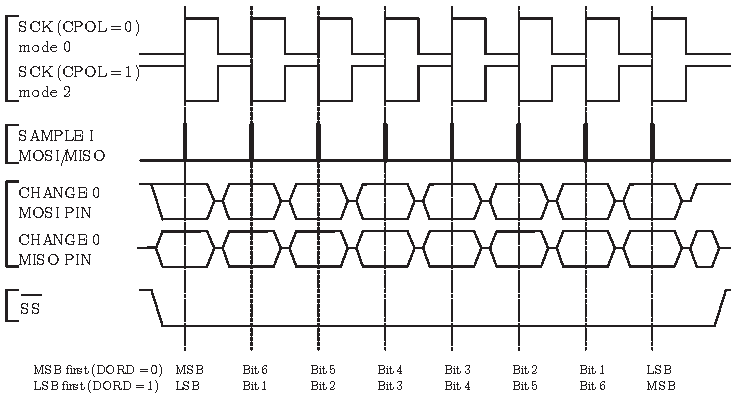
\includegraphics{spi_cpha-0}
    \end{center}
    \fullcite[168]{atmel13:spi-cpha0}
\end{figure}

Ο μικροελεγκτής ATmega238P υποστηρίζει εγγενώς το δίαυλο SPI καθώς διαθέτει
κύκλωμα αφιερωμένο κύκλωμα. Υποστηρίζει και τις τέσσερις ρυθμίσεις λειτουργίας
βάσει συνδυασμού πολικότητας-φάσης με δυνατότητα επιλογής της σειράς αποστολής
των \te{bit} (πλέον ή λιγότερο σημαντικό \te{bit}) ενώ η συχνότητα του ρολογιού
μπορεί να φτάνει μέχρι το μισό της συχνότητας του ρολογιού συστήματος. Οι
επιλογές αυτές γίνονται δια μέσω του καταχωρητή SPCR (\te{SPI Control Register})
\parencite[169]{atmel13}. Παρότι υποστηρίζεται, επιλέγεται η μη αξιοποίηση
διακοπής ως αποτέλεσμα αποστολής\slash{}λήψης κάθε \te{Byte}, αλλά, αντιθέτως, η
αναμονή μέχρι την ενεργοποίηση της ένδειξης SPIF (\te{SPI Interrupt Flag}) του
καταχωρητή SPSR (\te{SPI Status Register}) από το υποκείμενο κύκλωμα
\parencite[167,170]{atmel13}.

Στο πλαίσιο της υλοποίησης, ο δίαυλος SPI χρησιμοποιείται για τη διασύνδεση με
το ολοκληρωμένο δικτυακής σύνδεσης (βλ. \nameref{sec:w5100}
σ.~\pageref{sec:w5100}) και την εξωτερική μνήμη \te{Flash},
ενώ ως λειτουργία χρησιμοποιείται η \te{SPI mode 0} (δηλαδή, CPOL = 0, CPHA = 0)
καθώς υποστηρίζεται και από τα δύο ολοκληρωμένα.
